\documentclass[12pt]{article}

% Define the version in this line
%  THE GITHUB ACTION DEPENDS ON THE EXACT FORMAT OF THIS LINE; DO NOT CHANGE ANY
%  PART OF THIS LINE OTHER THAN THE VERSION NUMBER WITHOUT FIRST READING THE
%  GITHUB ACTION FILE
\newcommand{\versionNumber}{0.0.35}

% Create code that will enable us to put
%         \filesum{\jobname}
% anywhere in the document to output an MD5 hash of the source file.
% This will allow us to check that the PDF is in sync with the LaTeX source
% file. Code from:
%     https://tex.stackexchange.com/questions/327515/how-to-include-a-hash-of-a-source-file-in-the-final-pdf-file
\usepackage{pdftexcmds}
\makeatletter
\ifx\pdf@filemdfivesum\undefined\def\pdf@filemdfivesum#{\mdfivesum file}\fi
\let\filesum\pdf@filemdfivesum
\makeatother

%%% include file for lectures

%% packages
\usepackage{etex}
\usepackage{amsmath}
\usepackage{amssymb}
\usepackage{amsthm}
\usepackage{amsfonts}
\usepackage{epsfig}
\usepackage{latexsym}
\usepackage{url}
\usepackage{ifthen}
\usepackage{comment}
\usepackage{enumerate}
\usepackage{multirow}
\usepackage[english]{babel}
\usepackage{texnansi}
\usepackage{textcomp}
\usepackage{color}
\usepackage{calc}
\usepackage[normalem]{ulem}
\usepackage{array}
\usepackage{booktabs}
\usepackage[margin=10pt,font=small,labelfont=bf]{caption}
\usepackage[hypertexnames=false,hyperfootnotes=false,bookmarks=false]{hyperref}
\usepackage{sectsty}

%% spacing
\usepackage{setspace}
\usepackage[margin=1in]{geometry}

% boolean to use Lucida Bright as the font
\provideboolean{lucidabr}
% uncomment to use Lucida
%\setboolean{lucidabr}{true}

%% pick the font
\ifthenelse{\boolean{lucidabr}}{%
  % Lucida Bright
  \usepackage{lucidabr}
}{%
  % following two use Helvetica Neue for text, Latin Modern for math
  \usepackage{lmodern}
 %%%% \usepackage{gtamachelveticaneue}
}

%% customize section titles
\allsectionsfont{\large\sffamily}
\makeatletter
\def\@seccntformat#1{\csname the#1\endcsname.\quad}
\makeatother

%% tikz/pgf packages
\usepackage{tikz}
\usepackage{pgfpages}
\usepackage{pgfplots}
\usepackage{pgfplotstable}
\usetikzlibrary{arrows,decorations,patterns,trees,matrix,calc,shapes}
%this is obsolete, but useful for compatibility
%\usetikzlibrary{snakes}

%% useful math macros
\newcommand{\field}[1]{\mathbb{#1}}
\newcommand{\N}{\field{N}} % natural numbers
\newcommand{\R}{\field{R}} % real numbers
\renewcommand{\Re}{\R} % real numbers
\newcommand{\Z}{\field{Z}} % integers
\newcommand{\1}{\mathbf{1}} % vector of all 1's
\newcommand{\0}{\mathbf{0}} % vector of all 0's
\newcommand{\I}[1]{\mathbf{1}_{\left\{#1\right\}}} % indicator function
\newcommand{\Inb}[1]{I_{#1}} % indicator function, no brackets
\newcommand{\tends}{{\rightarrow}} % arrow for limits
\newcommand{\ra}{{\rightarrow}} % abbreviation for right arrow
\newcommand{\PR}{\mathsf{P}} % probability
\newcommand{\E}{\mathsf{E}} % expectation
\newcommand{\defeq}{\triangleq}
\newcommand{\subjectto}{\text{subject to}} % subject to
\newcommand{\ip}[2]{\langle #1, #2\rangle} % inner product

%% math operators
\DeclareMathOperator{\PV}{\text{PV}}
\DeclareMathOperator{\inter}{\textbf{int\,}}
\DeclareMathOperator{\relint}{\textbf{relint\,}}
\DeclareMathOperator{\dom}{\textbf{dom\,}}
\DeclareMathOperator{\cl}{\textbf{cl\,}}
\DeclareMathOperator{\conv}{\textbf{conv\,}}
\DeclareMathOperator{\card}{\textbf{card}}
\DeclareMathOperator{\aff}{\textbf{aff\,}}
\DeclareMathOperator{\var}{\text{Var}}
\DeclareMathOperator{\Var}{\text{Var}}
\DeclareMathOperator{\cov}{\text{Cov}}
\DeclareMathOperator{\sgn}{\text{sgn}}
\DeclareMathOperator{\TV}{\text{TV}}
\DeclareMathOperator{\BV}{\mathrm{BV}}
\DeclareMathOperator{\NBV}{\mathrm{NBV}}
\DeclareMathOperator*{\argmin}{\text{argmin}}
\DeclareMathOperator*{\argmax}{\text{argmax}}
\newcommand\minimize{\mathop{\text{minimize}}\limits}
\newcommand\maximize{\mathop{\text{maximize}}\limits}
\newcommand{\im}{\text{im\,}}
% redfine these to get the font right
\renewcommand{\ker}{\text{ker\,}}
\renewcommand\max{\mathop{\text{max}}\limits}
\renewcommand\min{\mathop{\text{min}}\limits}
\renewcommand\lim{\mathop{\text{lim}}\limits}
\renewcommand\log{\mathop{\text{log}}\limits}
\renewcommand\exp{\mathop{\text{exp}}\limits}
\renewcommand\sup{\mathop{\text{sup}}\limits}
\renewcommand\inf{\mathop{\text{inf}}\limits}
\renewcommand\sin{\mathop{\text{sin}}\limits}
\renewcommand\cos{\mathop{\text{cos}}\limits}
\renewcommand\tan{\mathop{\text{tan}}\limits}

%% some caligraphic symbols
\newcommand{\Ascr}{{\mathcal A}}
\newcommand{\Bscr}{{\mathcal B}}
\newcommand{\Cscr}{{\mathcal C}}
\newcommand{\Dscr}{{\mathcal D}}
\newcommand{\Escr}{{\mathcal E}}
\newcommand{\Fscr}{{\mathcal F}}
\newcommand{\Gscr}{{\mathcal G}}
\newcommand{\Hscr}{{\mathcal H}}
\newcommand{\Iscr}{{\mathcal I}}
\newcommand{\Jscr}{{\mathcal J}}
\newcommand{\Kscr}{{\mathcal K}}
\newcommand{\Lscr}{{\mathcal L}}
\newcommand{\Mscr}{{\mathcal M}}
\newcommand{\Nscr}{{\mathcal N}}
\newcommand{\Oscr}{{\mathcal O}}
\newcommand{\Pscr}{{\mathcal P}}
\newcommand{\Qscr}{{\mathcal Q}}
\newcommand{\Rscr}{{\mathcal R}}
\newcommand{\Sscr}{{\mathcal S}}
\newcommand{\Tscr}{{\mathcal T}}
\newcommand{\Uscr}{{\mathcal U}}
\newcommand{\Vscr}{{\mathcal V}}
\newcommand{\Wscr}{{\mathcal W}}
\newcommand{\Xscr}{{\mathcal X}}
\newcommand{\Yscr}{{\mathcal Y}}
\newcommand{\Zscr}{{\mathcal Z}}

%% abstract, table, figure names
\renewcommand{\figurename}{\normalfont\sffamily\bfseries Figure}
\renewcommand{\tablename}{\normalfont\sffamily\bfseries Table}

%% other customizations
\newcommand{\emailhref}[1]{\href{mailto:#1}{\tt #1}} % hyperlinked email address

%% always use 'stealth' arrows
\tikzstyle{every picture} += [>=stealth]

%% styles for figures
\tikzset{axis/.style={semithick, line join=miter}}

%% setup some layers
\pgfdeclarelayer{background}
\pgfdeclarelayer{foreground}
\pgfsetlayers{background,main,foreground}

%% table defaults
\pgfplotstableset{%
  font=\small,
  every head row/.style={before row=\toprule[1pt], after row=\midrule},
  every last row/.style={after row=\bottomrule[1pt]}}

%% pstricks ncline functionality
\newcommand{\tikznode}[2]{%
  \tikz[remember picture,baseline]%
  \node[anchor=base,inner sep=0pt] (#1) {#2};%
}
\newcommand{\tikznodefull}[3]{%
  \tikz[remember picture,baseline]%
  \node[anchor=base,inner sep=0pt,#2] (#1) {#3};%
}
\newcommand{\tikzcoord}[1]{%
  \tikz[remember picture,overlay,baseline=-0.5ex]%
  \node [coordinate] (#1) {};%
}
\newcommand{\tikzline}[3]{%
  \tikz[remember picture,overlay,baseline]%
    \draw [#1] (#2) to (#3);%
}

% a colored box around text
\newcommand{\tikznodebox}[2]{%
  \tikz[baseline]%
  \node[anchor=base,inner sep=0pt,#1] {#2};
}

%% spacing
\newcommand{\skipline}{\vspace{\baselineskip}}

%% macro for course name
\def\coursename#1{%
  \def\ctemp{#1}%
  \ifx\ctemp\@empty
  \def\insertcoursename{}
  \else
  \def\insertcoursename{\ignorespaces#1}
  \fi
}
\coursename{}

%% macro for the title

\makeatletter
\renewcommand{\maketitle}{\par%
  \newpage
  \global\@topnum\z@
  \null
  \vspace*{-2.5cm}
  \vskip 2em%
  \includegraphics[height=0.3in]{cbs-logo-horizontal}
  \hfill
  \parbox[b]{1.95in}{\noindent\bfseries\sffamily \insertcoursename \\
    \hskip 200pt}% \@date}
  \begin{center}
    {\large\bfseries\sffamily \@title}
  \end{center}
}
\makeatother

%% indentation, etc.
\setlength{\parindent}{0pt}
\setlength{\parskip}{10pt}

%% course name
%\coursename{B6101 Business Analytics}

%% date
%\date{Spring 2014}

%% author
%\author{Professor: Ciamac Moallemi}

%%% Local Variables:
%%% mode: latex
%%% TeX-master: 'shared
%%% End:


\title{~\\~\\ \Large BA Excel Add-In User's Manual (Version~\versionNumber)}

\usepackage{titlesec}
\titleformat*{\section}{\sffamily\Large\bfseries}
\titleformat*{\subsection}{\sffamily\large\bfseries}
\titleformat*{\subsubsection}{\sffamily\large\bfseries}

\setcounter{tocdepth}{3}
\begin{document}

\maketitle
\vspace{-1cm}
{ \center{{\tiny \color{white} Manual version: \filesum{\jobname}}} }

\tableofcontents

\clearpage

%\section{Preliminaries}\label{prelim}
%
%
%
%The BA Excel add-in \underline{only runs under Windows}, so Mac users will need to be able to boot into Windows. There is no license associated with this add-in so you may keep it after the course and continue to use it. The add-in extends the functionality of Excel to provide several additional analytic tools such as logistic regression, k-nearest neighbors, ROC curves and Monte Carlo simulation.
%
%%\medskip
%%{\bf This Section:} This section provides an introduction
%%\texttt{logistic\_regression\_practice.xlsx}.
%%\medskip
%
%
%\subsection{Download}\label{install}
%
%
%
%To install the BA Excel Add-In, download the installation package from the course's canvas page:
%\begin{itemize}
%\item cbs\_ba\_setup\_32bit.exe   (if you have 32-bit Excel)
%\item cbs\_ba\_setup\_64bit.exe  (if you have 64-bit Excel)
%\end{itemize}
%
%You may need to check whether your Excel is 32-bit or 64-bit:
%\begin{itemize}
%	\item Excel 2003-2007: These versions of Excel are 32-bit
%	\item Excel 2010: File tab from Excel > Help
%	\item Excel 2013: File tab from Excel > Account > About Excel
%\end{itemize}
%
%It is important to note that Excel may be either 32-bit or 64-bit even though you have 64-bit Windows. Most people have 32-bit Excel installed. If you see a screen of binary gibberish after installation, you picked the wrong installation package.
%
%\subsection{Installation}
%
%The installation package, cbs\_ba\_setup\_32bit.exe (or cbs\_ba\_setup\_64bit.exe), will install the BA add-in so that it is loaded automatically every time Excel is started. Just double click the installation package and follow the instructions.
%
%To check whether the add-in is installed successfully, look for an "Add-Ins" tab that should have appeared on the top after "View". Click on "Add-Ins". Look for a drop-down menu named "CBS\_ba Help". If you see this menu, you have successfully installed the add-in. The drop-down menu contains links to a Catalog containing example usage of each of the functions provided in the add-in, and a Simulation example. 
%%To check whether the add-in is installed successfully, find ``Excel Options | Add-ins'' and select ``Excel add-ins'' at the bottom and click ``Go''. If ``cbs\_ba'' item is checked, the add-in is successfully installed. 
%
%
%\subsection{Troubleshooting Monte Carlo Simulation}
%
%If you experience issues with running Monte Carlo simulations with the add-in, please try the following:
%
%Make sure that you see the dialog box that says  ``CBS Business Analytics Excel add-in''`` when the add-in is launched. If not, the add-in was not properly installed.
%
%In some instances, other add-ins can interfere with the CBS BA add-in. Try disabling other add-ins by looking under ``Excel Options | Add-ins''. One particular add-in that is known to be problematic is the ``Send to Bluetooth'' add-in. You'll need to make sure to leave the Solver add-in enabled.
%
%If you try all of these options and the add-in still does not work, please contact your instructor.
%
%\medskip
%
%\newpage
\section{The BA Add-In Functions}\label{list}

\subsection{Linear Regression Functions}

\subsubsection{LinearRegTrain}\label{regtrain}


\textit{The example illustrated below is available on the}  \href{https://www8.gsb.columbia.edu/bizanalytics/excel-add-in/multiplatform#h-4}{ \textit{add-in webpage}}
 \textit{by downloading the Linear and Logistic Regression file and going to the linearReg sheet.}

\textbf{LinearRegTrain} is an array function that allows you to estimate the coefficients $(\beta_0,\beta_1,...,\beta_K)$ of a regression equation of the form
\[
\texttt{Y}=\beta_0+\beta_1 \texttt{Var1}+\beta_2 \texttt{Var2} +...+ \beta_K \texttt{VarK}+\epsilon,
\]
using observed data on the independent variables $(\texttt{Var1},\texttt{Var2},...,\texttt{VarK})$ and on the dependent variable $\texttt{Y}$. This function outputs the estimated coefficients, the standard errors, the associated p-values, and the R-squared of the regression.

We illustrate how this function works with a dataset that contains $10$ observations of $3$ independent variables (\texttt{Var1},\texttt{Var2},\texttt{Var3}) and the dependent variable \texttt{Y}.

To use the function:
\begin{enumerate}
\item Select the cell where you want to display the output (\texttt{H3} in the example) and call the function by typing \texttt{=LinearRegTrain(} and then clicking on the $\boldsymbol{f_x}$ symbol next to the formula bar. (Alternatively, you can call the function by clicking on the  $\boldsymbol{f_x}$ symbol first, which will display a menu of all available functions, and then clicking on \texttt{LinearRegTrain}.)

\medskip

\centerline{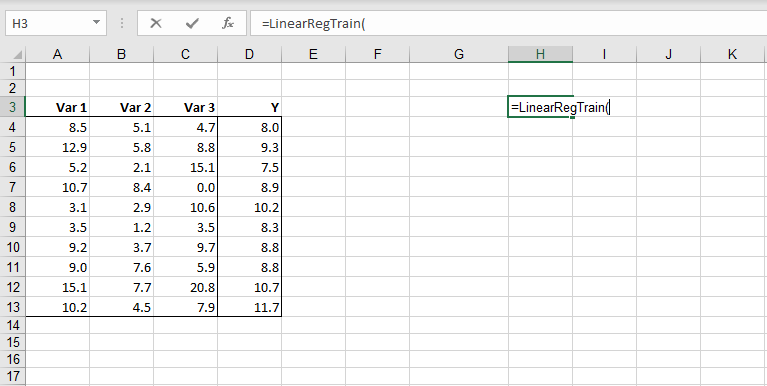
\includegraphics[width=6in]{figures/LinRegTrain1}}

\medskip

\item When you call the function, the window \texttt{Function Arguments} will appear. Follow the instructions to populate the input fields, then click \texttt{OK}.

\medskip

\centerline{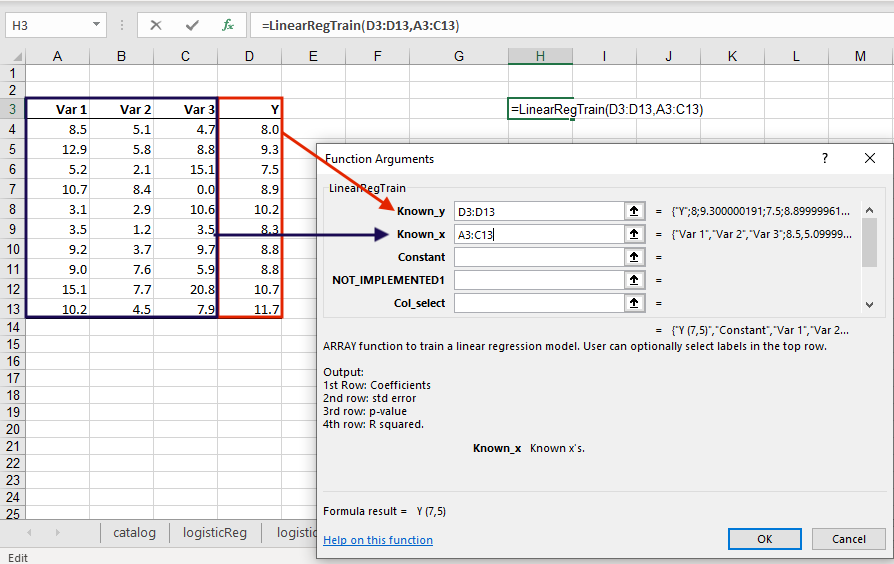
\includegraphics[width=6in]{figures/LinRegTrain2}}

\medskip

\item The string \texttt{Y(7,5)} will appear in cell \texttt{H3}, where \texttt{Y} is the name of the variable in cell \texttt{D3}. This indicates that you should select an output array of \texttt{7} rows and \texttt{5} columns. Select the output array starting from cell \texttt{H3} as the next figure shows.

\medskip

\centerline{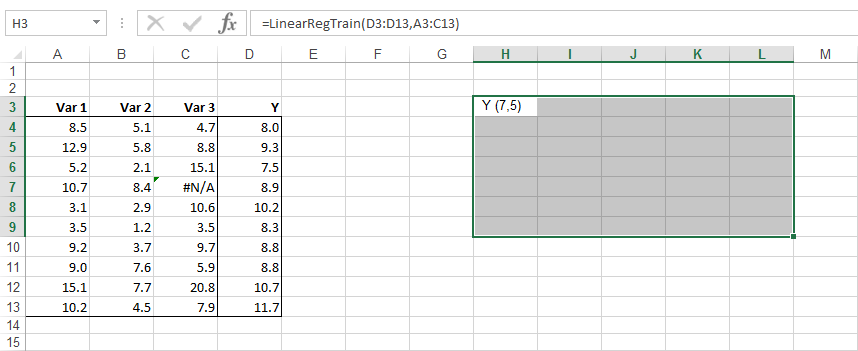
\includegraphics[width=6in]{figures/LinRegTrain3New}}

\medskip

\item Position the cursor in the formula bar, and press \texttt{Ctrl+Shift+Enter} to display the output. \textit{Remark: for recent versions of Excel, this step is not necessary.}

\medskip

\centerline{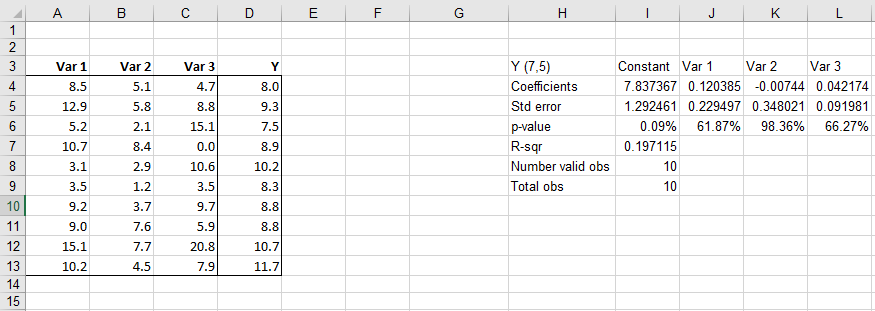
\includegraphics[width=6in]{figures/LinRegTrain4}}

\medskip
\end{enumerate}

The second row of the output contains the estimates of the coefficients: the column (\texttt{Constant}) refers to the coefficient $\beta_0,$ while the columns (\texttt{Var1},\texttt{Var2},\texttt{Var3}) refer to the coefficients $(\beta_1,\beta_2,\beta_3)$ respectively. In the following rows we have standard errors and p-values of the estimates as well as the $R^2$ of the regression. The last two rows contain the number of valid observations and the total number of observations respectively.

You can also format the output to display only three decimals and to display percentages.


\paragraph{Optional Input: Col\_select.} The optional input \texttt{Col\_select} allows you to specify which variables you want to include in your regression. For example, the configuration below runs a logistic regression with only \texttt{Var1} and \texttt{Var3} as independent variables.
\medskip

\centerline{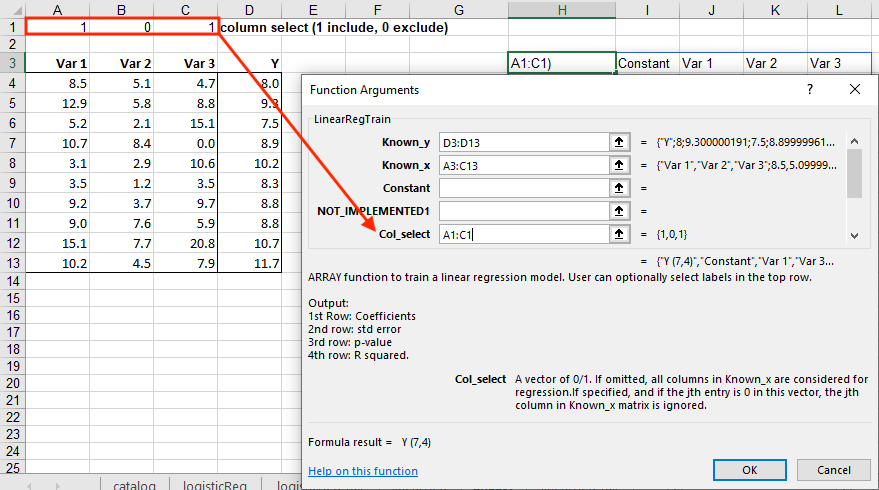
\includegraphics[width=6in]{figures/LinRegTrainOptional1}}

\medskip
\iffalse
 This function outputs:
\begin{enumerate}[i)]
\item $(\hat \beta_0,\hat \beta_1,\hat \beta_2,...,\hat \beta_K)$ - an array of length $K+1$ that contains the estimates of all coefficients.
\item $(se(\hat \beta_0),se(\hat \beta_1),se(\hat \beta_2),...,se(\hat \beta_K))$ - an array of length $K+1$ that contains the standard errors of the coefficients.
\item $(p_0,p_1,p_2,...,p_K)$ - an array of length $K+1$ that contains the p-values of a t-test for each coefficient. That is, for every $i=0,1,2,...,K$, $p_i$ is the p-value of the following t-test:
\begin{align*}
H_0&: \beta_i=0\\
H_1&: \beta_i\neq 0.
\end{align*}
\item The $R^2$ of the regression; the number of valid observations; the number of total observations.
\end{enumerate}
\fi
%$\beta_0,\beta_1,\beta_2$ and $\beta_3$

\subsubsection{LinearRegPredict}

\textit{The example illustrated below is available on the}  \href{https://www8.gsb.columbia.edu/bizanalytics/excel-add-in/multiplatform#h-4}{ \textit{add-in webpage}}
 \textit{by downloading the Linear and Logistic Regression file and going to the linearReg sheet.}

\textbf{LinearRegPredict} uses the coefficients $(\beta_0^{e},\beta_1^{e},...,\beta_K^{e})$ that we estimate with \textbf{LinearRegTrain} and the data on the independent variables $(\texttt{Var1},\texttt{Var2},...,\texttt{VarK})$ to compute a prediction for the dependent variable using the formula
\[
\texttt{Y}^{\texttt{p}}=\beta_0^{e}+\beta_1^{e} \texttt{Var1}+\beta_2^{e} \texttt{Var2} +...+ \beta_K^{e} \texttt{VarK}.
\]
For example, using the coefficients that we estimated in the \textbf{LinearRegTrain} example we would predict \texttt{Y} using the following formula
\[
\texttt{Y}^{\texttt{p}}=7.854+0.114  \texttt{Var1}+0.023 \texttt{Var2}+ 0.034 \texttt{Var3},
\]
which, for the first observation, yields a prediction of
\[
9.1001=7.854+0.114*8.5+0.023*5.1+ 0.034*4.7.
\]
To use the function:
\begin{enumerate}
\item Select the first cell in which you want the output to be displayed; call the function by typing \texttt{=LinearRegPredict(} in the formula bar and then pressing the $\boldsymbol{f_x}$ symbol next to the formula bar.

\medskip

\centerline{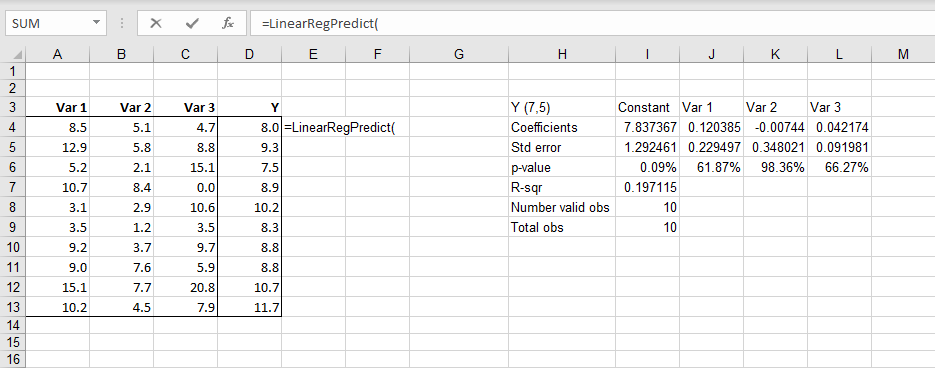
\includegraphics[width=6in]{figures/LinRegPred1}}

\medskip

\item Follow the instructions to populate the input fields, as demonstrated in the figure below, then click \texttt{OK}.

\medskip

\centerline{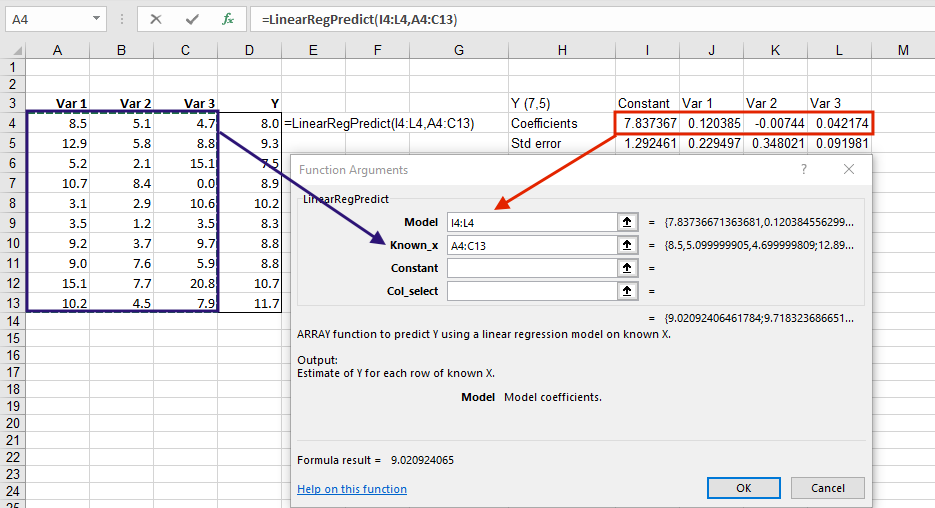
\includegraphics[width=6in]{figures/LinRegPred2}}

\medskip

\item Remember that this is an array function. Select the column in which you want the output to be displayed: this should be a column of the same length as the number of observations that will contain the predictions associated to each observation. In the figure below, we have 10 observations and we select cells \texttt{E4:E13}.

\medskip

\centerline{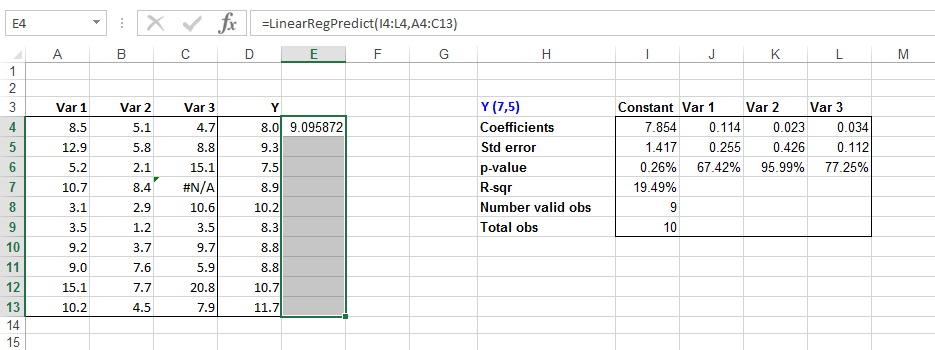
\includegraphics[width=6in]{figures/LinRegPred3New}}

\medskip

\item Position the cursor in the formula bar, and press \texttt{Ctrl+Shift+Enter} to display the predictions. You can also add a title (for example ``LinearRegPredict'') to the output-column and format the output-cells to display only the first 3 decimals, as in the figure below. \textit{Remark: for recent versions of Excel, this step is not necessary.}

\medskip

\centerline{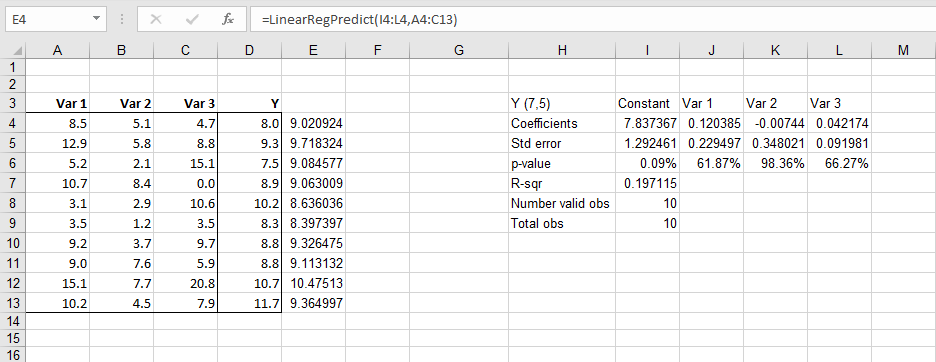
\includegraphics[width=6in]{figures/LinRegPred4}}

\medskip

\end{enumerate}

\paragraph{Optional Input: Col\_select.} See explanation at the end of Section \ref{regtrain}.

%\paragraph{Optional Input: Row\_weight.} The optional input \texttt{Row\_weight} allows you to specify a weight for each row. The default weight is 1 for each row. To specify the weights from the column ``row weight'' type \texttt{F4:F13} in the \texttt{Row\_weight} field of the function input dialog box.
%\medskip

%\centerline{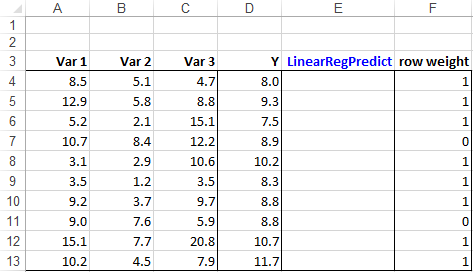
\includegraphics[width=3.2in]{figures/LinRegPreda1}}

%\medskip

%\newpage

\subsection{Logistic Regression Functions}

\subsubsection{LogisticRegTrain}\label{logregtrain}

\textit{The example illustrated below is available on the}  \href{https://www8.gsb.columbia.edu/bizanalytics/excel-add-in/multiplatform#h-4}{ \textit{add-in webpage}}
 \textit{by downloading the Linear and Logistic Regression file and going to the logisticReg sheet.}

\textbf{LogisticRegTrain} is an array function that allows you to estimate the coefficients $(\beta_0,\beta_1,...,\beta_K)$ of a logistic regression model
using observed data on the independent variables $(\texttt{Var1},\texttt{Var2},...,\texttt{VarK})$ and on the dependent variable $\texttt{Y}$. Note that the dependent variable in a logistic regression must be binary, i.e. it must take values $0$ or $1$. This function outputs the estimated coefficients, the standard errors, and the associated p-values. This function allows you to estimate the probability that the dependent variable is equal to 1 as
\[
Pr(\text{dependent variable equals one})=\frac{\exp(w)}{1+\exp(w)},
\]
with
\[
w=\beta_0+\beta_1 \texttt{Var1}+\beta_2 \texttt{Var2} +...+ \beta_K \texttt{VarK}.
\]

We illustrate how this function works with a dataset that contains $18$ observations of $3$ independent variables (\texttt{Var1},\texttt{Var2},\texttt{Var3}) and the dependent variable \texttt{Y}.

To use the function:
\begin{enumerate}
\item Select the cell where you want to display the output (\texttt{H3} in the example) and call the function by typing \texttt{=LogisticRegTrain(} and then clicking on the $\boldsymbol{f_x}$ symbol next to the formula bar. (Alternatively, you can call the function by clicking on the  $\boldsymbol{f_x}$ symbol first, which will display a menu of all available functions, and then clicking on \texttt{LogisticRegTrain}.)

\medskip

\centerline{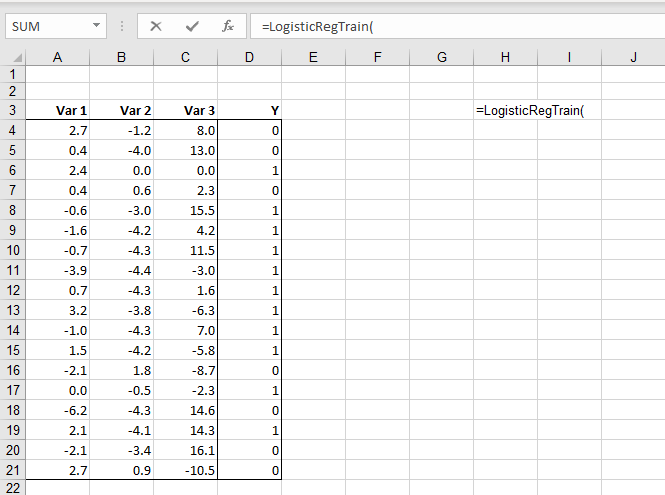
\includegraphics[width=6in]{figures/LogRegTrain1}}

\medskip

\item When you call the function, the window \texttt{Function Arguments} will appear. Follow the instructions to populate the input fields, then click \texttt{OK}.

\medskip

\centerline{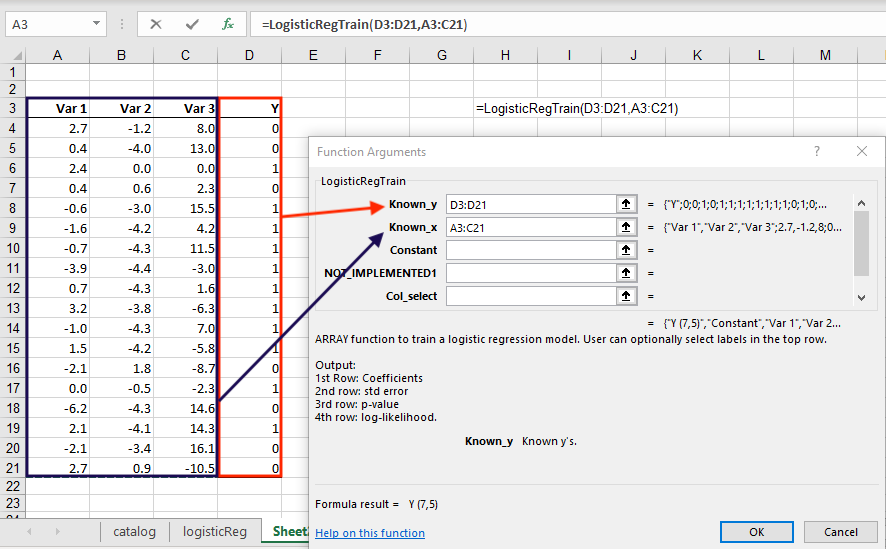
\includegraphics[width=6in]{figures/LogRegTrain2}}

\medskip

\item  The string \texttt{Y(7,5)} will appear in cell \texttt{H3}, where \texttt{Y} is the name of the variable in cell \texttt{D3}. This indicates that you should select an output array of \texttt{7} rows and \texttt{5} columns. Select the output array starting from cell \texttt{H3} as the next figure shows.

\medskip

\centerline{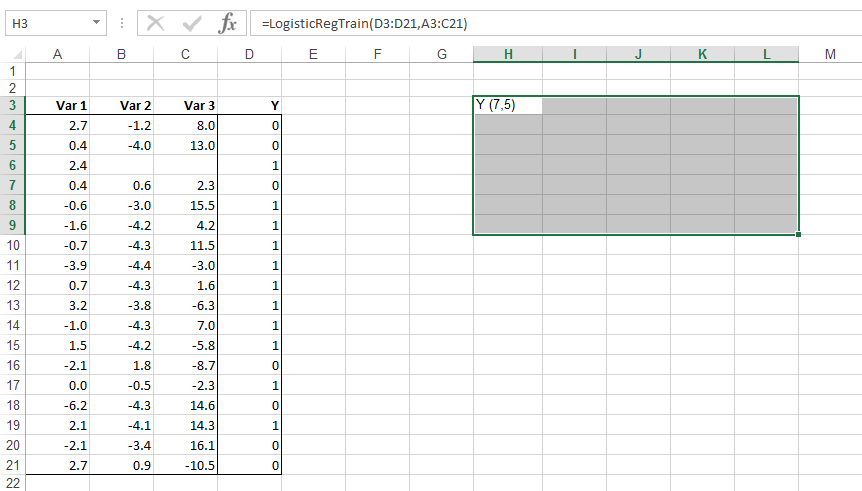
\includegraphics[width=6in]{figures/logreg3New}}

\medskip

\item Position the cursor in the formula bar, and press \texttt{Ctrl+Shift+Enter} to display the output. \textit{Remark: for recent versions of Excel, this step is not necessary.}

\medskip

\centerline{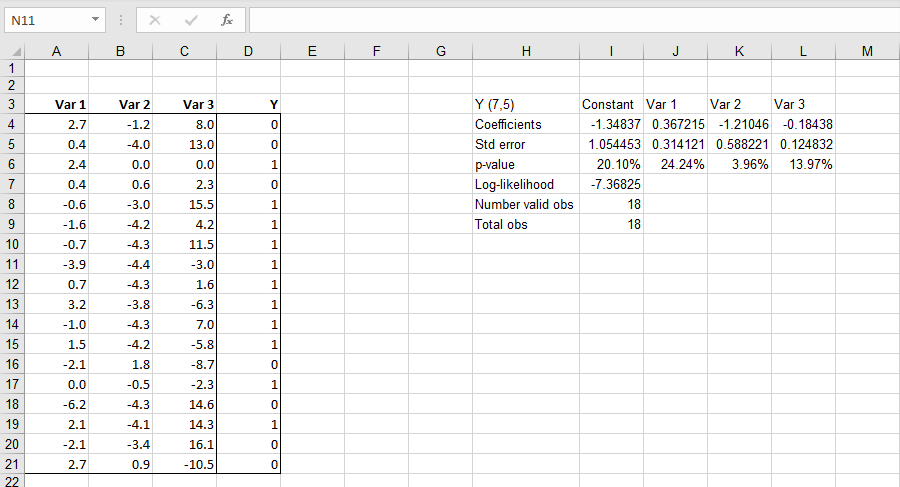
\includegraphics[width=6in]{figures/LogRegTrain4}}

\medskip
\end{enumerate}

The second row of the output contains the estimates of the coefficients: the column (\texttt{Constant}) refers to the coefficient $\beta_0,$ while the columns (\texttt{Var1},\texttt{Var2},\texttt{Var3}) refer to the coefficients $(\beta_1,\beta_2,\beta_3)$ respectively. In the following rows we have standard errors and p-values of the estimates. The last two rows contain the number of valid observations and the total number of observations respectively.

You can also format the output to display only three decimals and to display percentages.

\paragraph{Optional Input: Col\_select.} The optional input \texttt{Col\_select} allows you to specify which variables you want to include in your regression. For example, the configuration below runs a logistic regression with only \texttt{Var1} and \texttt{Var3} as independent variables.
\medskip

\centerline{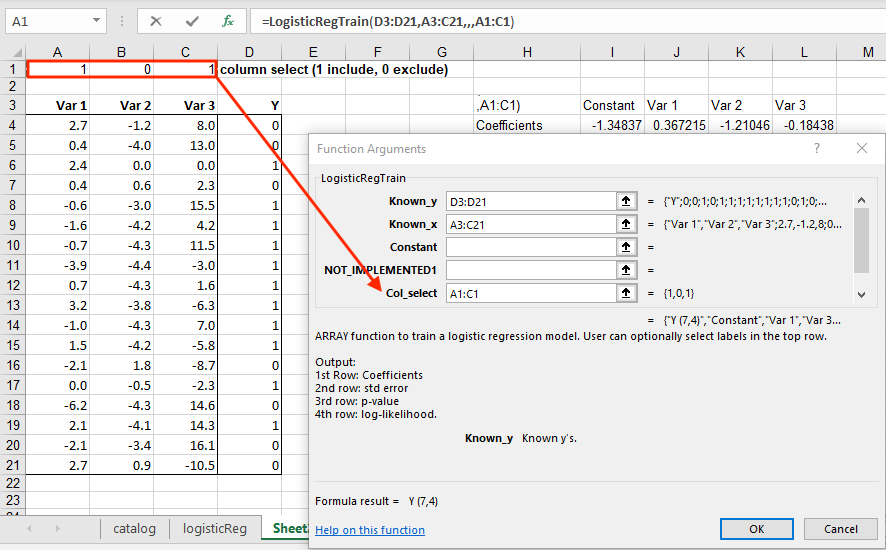
\includegraphics[width=6in]{figures/LogRegTrainOptional1}}

\medskip

\subsubsection{LogisticRegPredict}

\textit{The example illustrated below is available on the}  \href{https://www8.gsb.columbia.edu/bizanalytics/excel-add-in/multiplatform#h-4}{ \textit{add-in webpage}}
 \textit{by downloading the Linear and Logistic Regression file and going to the logisticReg sheet.}

\textbf{LogisticRegPredict} uses the coefficients $(\beta_0^{e},\beta_1^{e},...,\beta_K^{e})$ that we estimate with \textbf{LogisticRegTrain} and the data on the independent variables $(\texttt{Var1},\texttt{Var2},...,\texttt{VarK})$ to compute a prediction $p$ for the probability that the dependent variable is equal to 1. The prediction is calculated in two steps:
\begin{itemize}
\item[(i)] Obtain the exponent $w$ of the logistic function as
\[
w=\beta_0^{e}+\beta_1^{e} \texttt{Var1}+\beta_2^{e} \texttt{Var2} +...+ \beta_K^{e} \texttt{VarK}.
\]
\item[(ii)] Calculate the probability that \texttt{Y}=1 as follows
\[
p=\frac{\exp(w)}{1+\exp(w)}.
\]
\end{itemize}

For example, using the coefficients that we estimated in the \textbf{LogisticRegTrain} example we would predict $p$  for the first observation in the example as follows
\[
w=-2.047+0.301 * 2.7- 1.432 * (-1.2) -0.207 * 8=-1.172
\]
and
\[
p=\frac{\exp(-1.172)}{1+\exp(-1.172)}=23.61\%
\]

To use the function:
\begin{enumerate}
\item Select the first cell in which you want the output to be displayed; call the function by typing \texttt{=LogisticRegPredict(} in the formula bar and then pressing the $\boldsymbol{f_x}$ symbol next to the formula bar.

\medskip

\centerline{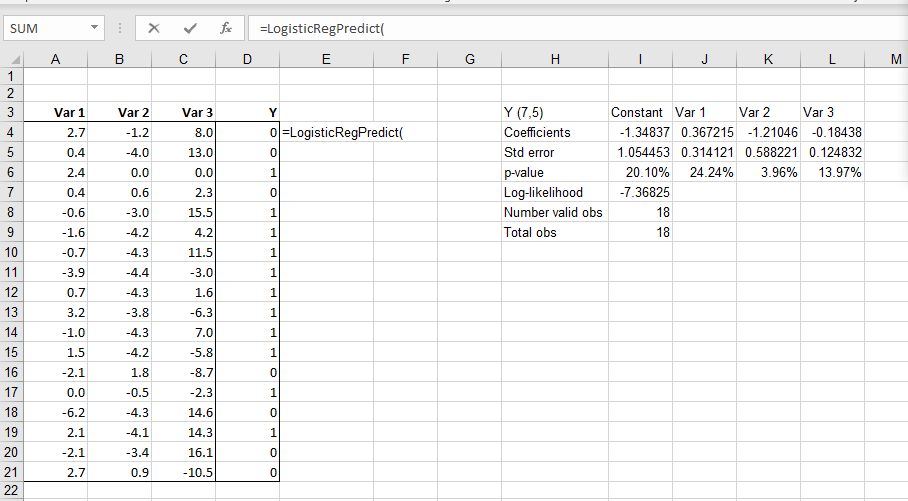
\includegraphics[width=6in]{figures/LogRegPred1}}

\medskip

\item Follow the instructions to populate the input fields, as demonstrated in the figure below, then click \texttt{OK}.

\medskip

\centerline{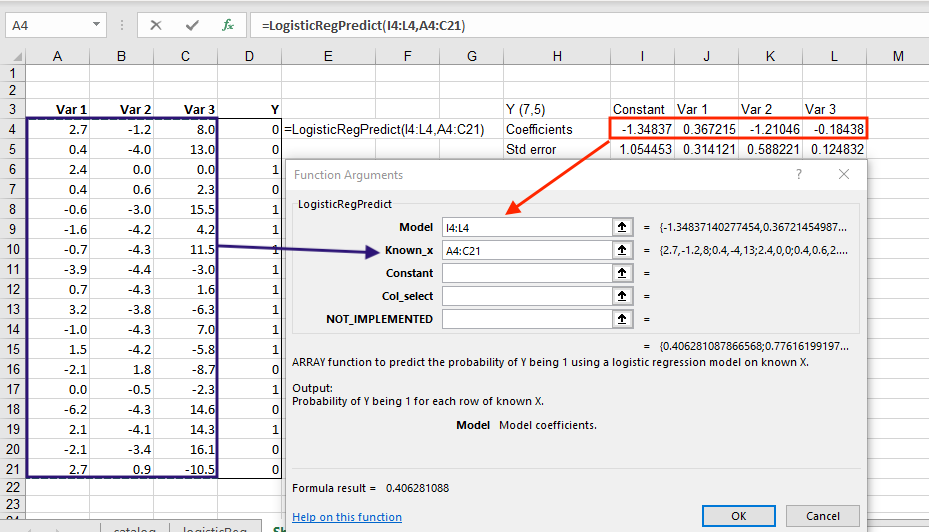
\includegraphics[width=6in]{figures/LogRegPred2}}

\medskip

\item Remember that this is an array function. Select the column in which you want the output to be displayed: this should be a column of the same length as the number of observations that will contain the predictions associated to each observation. In the figure below, we have 18 observations and we select cells \texttt{E4:E21}.

\medskip

\centerline{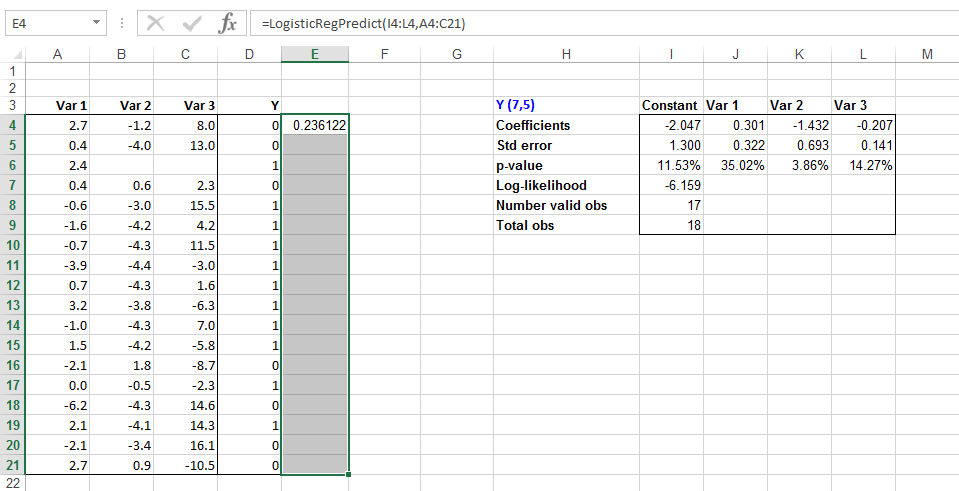
\includegraphics[width=6in]{figures/logpred3New}}

\medskip

\item Position the cursor in the formula bar, and press \texttt{Ctrl+Shift+Enter} to display the predictions. You can also add a title (for example ``LogisticRegPredict'') to the output-column and format the output-cells to display percentages, as in the figure below. \textit{Remark: for recent versions of Excel, this step is not necessary.}

\medskip

\centerline{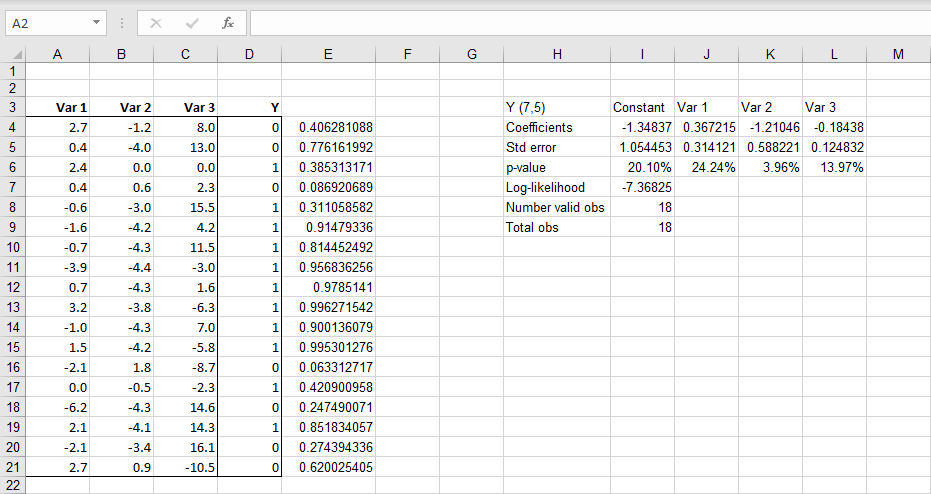
\includegraphics[width=6in]{figures/LogRegPred4}}

\end{enumerate}

\paragraph{Optional Input: Col\_select.} See explanation at the end of Section \ref{logregtrain}.

%\paragraph{Optional Input: Row\_weight.} The optional input \texttt{Row\_weight} allows you to specify integer weight for each row. The default weight is 1 for each row. To specify the row weights from the column ``row select'' type \texttt{F4:F21} in the \texttt{Row\_weight} field of the function input dialog box.
%\medskip

%\centerline{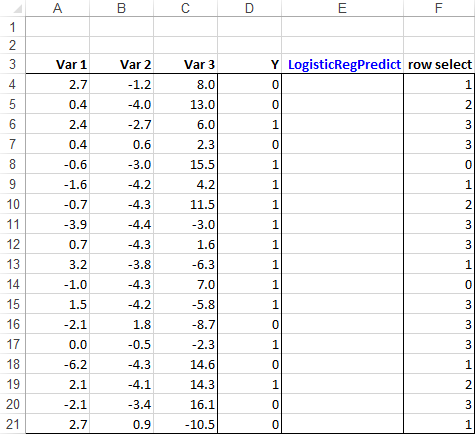
\includegraphics[width=4in]{figures/logpreda1}}

%\medskip

\subsection{K-Nearest Neighbor Functions (Content-based)}

\textit{Tip:} The functions in this section do content-based prediction, which means that they predict a score (or rating) based on other known attributes of content. The dependent variable (score or rating) and the independent variables (other attributes) are distinct, and in general you need information on both to be able to use these functions.

\subsubsection{knn\_in}

\textit{The example illustrated below is available on the}  \href{https://www8.gsb.columbia.edu/bizanalytics/excel-add-in/multiplatform#h-4}{ \textit{add-in webpage}}
 \textit{by downloading the Classification, KNN, Misc file and going to the knn sheet.}

\textbf{knn\_in} applies the \texttt{k}-nearest neighbor algorithm to make predictions within a specified sample. The inputs of the function are: the parameter \texttt{k} of nearest neighbor to match; the known variables $(\texttt{Var1},\texttt{Var2},...,\texttt{VarM})$, on the basis of which the observations are matched; the known outcomes $\texttt{Y}$. The nearest neighbor to a given observation are the observations which have minimum Euclidean distance
\[
d(i,j)=\sqrt{(\texttt{Var1}_i-\texttt{Var1}_j)^2+(\texttt{Var2}_i-\texttt{Var2}_j)^2+...+(\texttt{VarM}_i-\texttt{VarM}_j)^2}
\]
and the prediction $p$ is computed as a simple average of the \texttt{k}-nearest neighbor outcomes
\[
p=\frac{\texttt{Y}_1+\texttt{Y}_2+...+\texttt{Y}_k}{k}.
\]

To use the function:
\begin{enumerate}
\item Write the parameter \texttt{k} in an empty cell, \texttt{k}=3 in the example below; select the first cell in which you want the output to be displayed; call the function by typing \texttt{=knn\_in(} in the formula bar and then pressing the $\boldsymbol{f_x}$ symbol next to the formula bar.

\medskip

\centerline{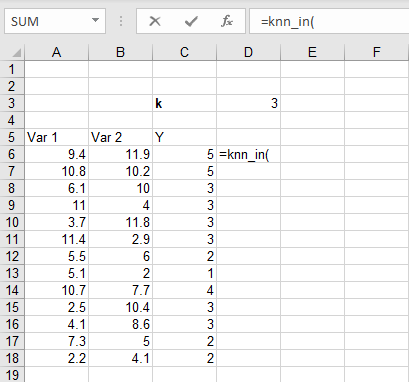
\includegraphics[width=2.2in]{figures/knnin1}}

\medskip

\item Follow the instructions to populate the input fields, as demonstrated in the figure below, then click \texttt{OK}.

\medskip

\centerline{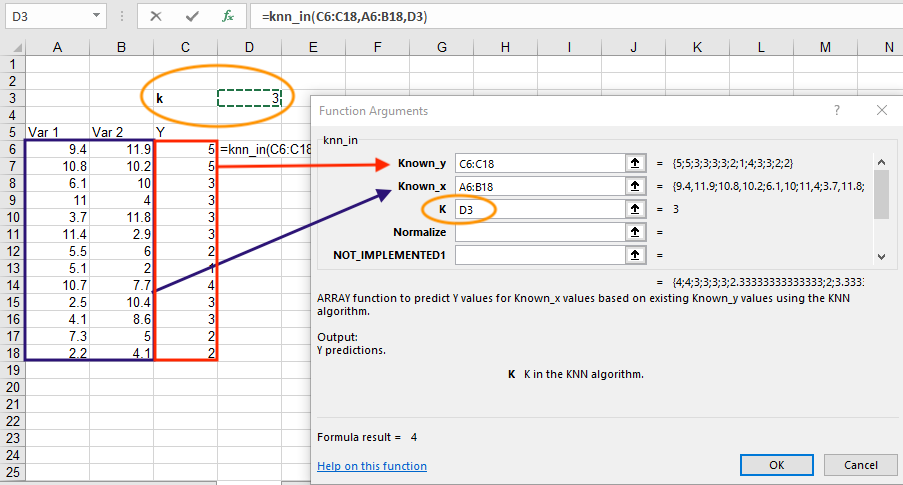
\includegraphics[width=5.5in]{figures/knnin2}}

\medskip

\item Remember that this is an array function. Select the column in which you want the output to be displayed: this should be a column of the same length as the number of observations. In the figure below, we selected cells \texttt{D6:D18}.

\medskip

\centerline{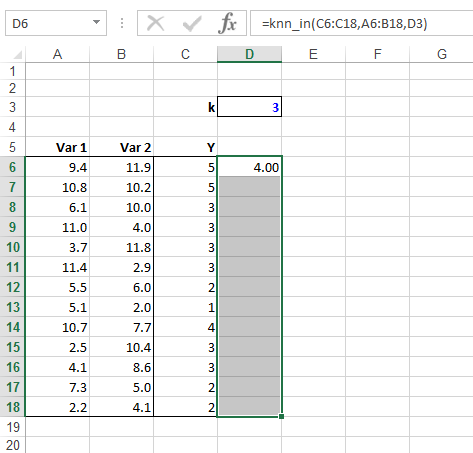
\includegraphics[width=2.5in]{figures/knnin3}}

\medskip

\item Position the cursor in the formula bar, and press \texttt{Ctrl+Shift+Enter} to display the predictions. You can also add a title (for example ``knn\_in predict'') to the output-column and format the output-cells to display only the first two decimals. \textit{Remark: for recent versions of Excel, this step is not necessary.}

\medskip

\centerline{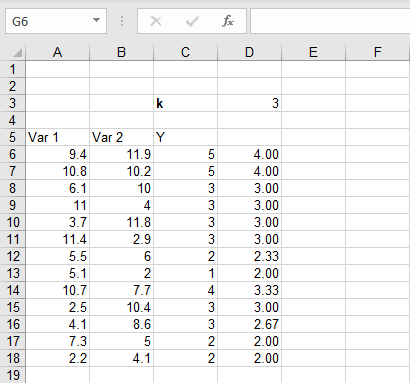
\includegraphics[width=2.2in]{figures/knnin4}}

\medskip
\end{enumerate}

\subsubsection{knn\_in\_rmse}

\textit{The example illustrated below is available on the}  \href{https://www8.gsb.columbia.edu/bizanalytics/excel-add-in/multiplatform#h-4}{ \textit{add-in webpage}}
 \textit{by downloading the Classification, KNN, Misc file and going to the knn\_full sheet.}

\textbf{knn\_in\_rmse} is a function that computes the Root Mean Squared Error (RMSE) for \text{k}-nearest neighbor predictions (as the ones you can obtain with \textbf{knn\_in}).


The inputs of the function are: the known variables $(\texttt{Var1},\texttt{Var2},...,\texttt{VarM})$ on the basis of which the observations are matched; the known outcomes $\texttt{Y}$; the parameter \texttt{k} for which we want to compute the RMSE of predictions.

For a given \texttt{k}, the error is computed as follows
\[
RMSE = \sqrt{\frac{(Y_1-p_1)^2+(Y_2-p_2)^2+...+(Y_N-p_N)^2}{N}},
\]
where $N$ is the total number of observations.

\textit{Note:} this is not an array function and can be evaluated in a single stand-alone cell, in which case it outputs the RMSE for a specified \text{k}. However, it is particularly useful when you want to compare RMSEs for different \text{k}. We will illustrate how to do this in the example below.

To use the function:
\begin{enumerate}
\item Write a list of parameters \texttt{k} for which you want to compute the RMSE, $\texttt{k}=1,2,...,10$ in the example below; select the cell next to the first value for \texttt{k}; call the function by typing \texttt{=knn\_in\_rmse(} in the formula bar and then pressing the $\boldsymbol{f_x}$ symbol next to the formula bar.

\medskip

\centerline{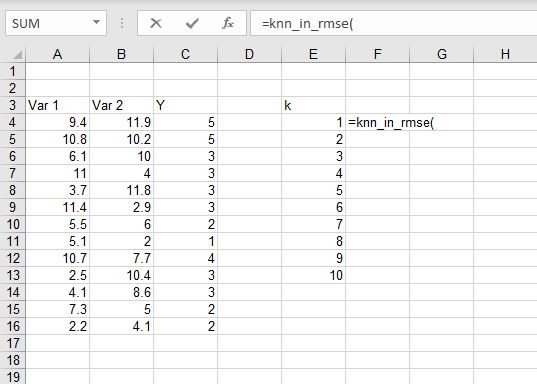
\includegraphics[width=3in]{figures/knnrmse1}}

\medskip

\item Input the references to the cells that contain the independent and dependent variable data, as in the figure below, then \textit{lock} the cell references with $\$$ signs. Input the reference of the cell that contains the first value for \texttt{k}, and make sure that this is \textit{not locked}. Then click \texttt{OK}.

\medskip

\centerline{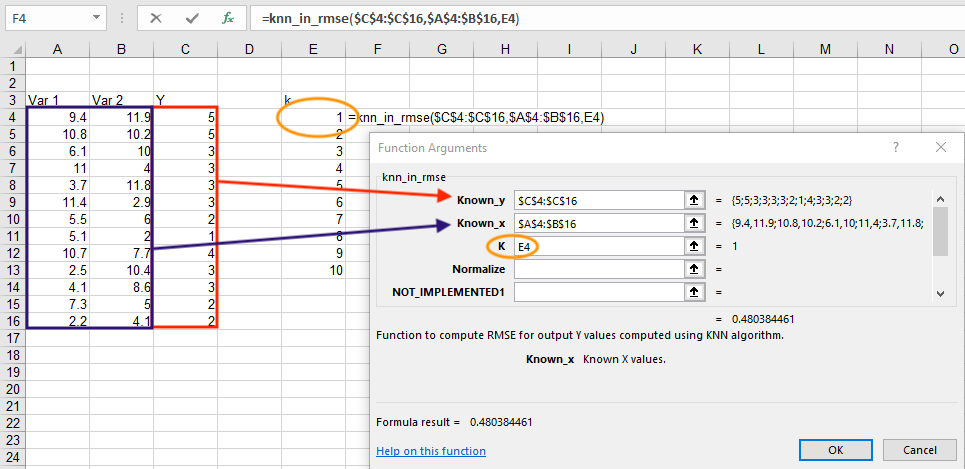
\includegraphics[width=5.5in]{figures/knnrmse2}}

\medskip

\item The function will display the output in the selected cell (\texttt{F4}). Copy the content of the cell down until cell \texttt{F13}, the formula will automatically update the calculation for every \texttt{k}. You can also format the output to display only three decimals.
\medskip

\centerline{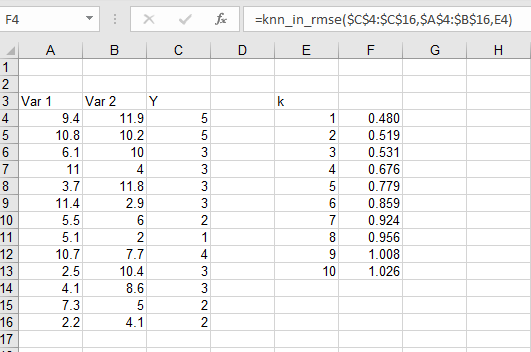
\includegraphics[width=2.6in]{figures/knnrmse3}}

\medskip
\end{enumerate}

\subsubsection{knn\_out}

\textit{The example illustrated below is available on the}  \href{https://www8.gsb.columbia.edu/bizanalytics/excel-add-in/multiplatform#h-4}{ \textit{add-in webpage}}
 \textit{by downloading the Classification, KNN, Misc file and going to the knn\_full sheet.}

\textbf{knn\_out} applies the-\texttt{k} nearest neighbor algorithm to make predictions on the outcome variable \texttt{Y} of a new set of observations using a known sample.

To use the function:
\begin{enumerate}
\item Write the parameter \texttt{k} in an empty cell, \texttt{k}=3 in the example below. Select the first cell in which you want the output to be displayed; call the function by typing \texttt{=knn\_out(} in the formula bar and then pressing the $\boldsymbol{f_x}$ symbol next to the formula bar.

\medskip

\centerline{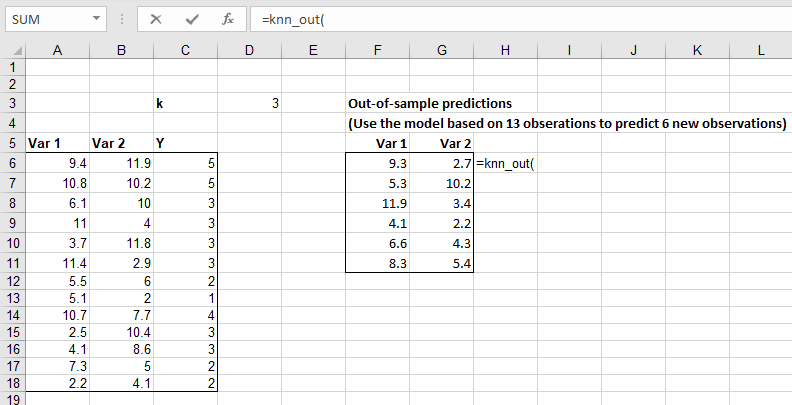
\includegraphics[width=5in]{figures/knnout1}}

\medskip

\item The function takes as inputs the new observations $X$, the old observations and the known outcomes, as well as the parameter \texttt{k}. Follow the instructions to populate the input fields, as demonstrated in the figure below, then click \texttt{OK}.

\medskip

\centerline{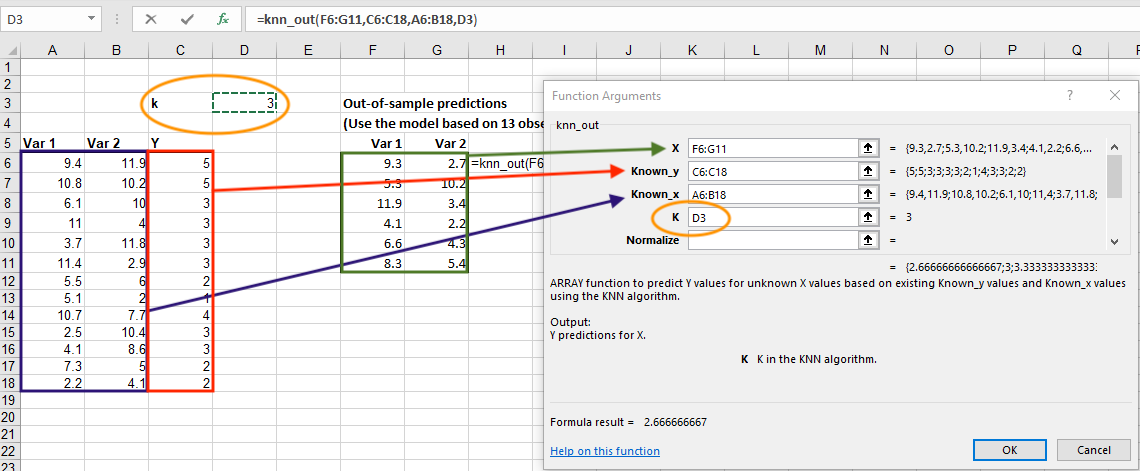
\includegraphics[width=5in]{figures/knnout2}}

\medskip

\item Remember that this is an array function. Select the column in which you want the output to be displayed: this should be a column of the same length as the number of new observations.

\medskip

\centerline{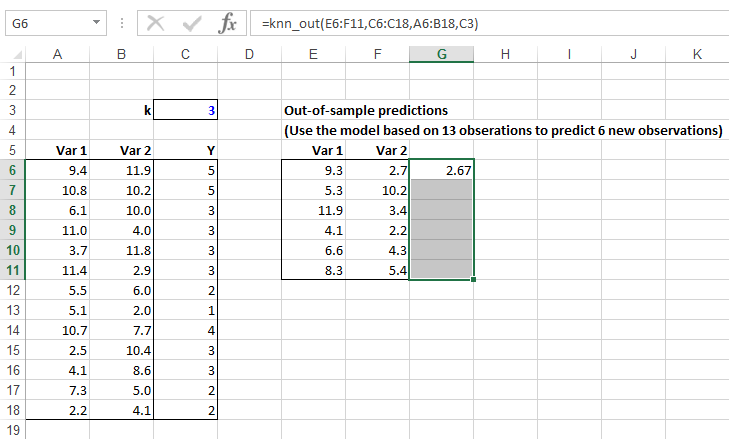
\includegraphics[width=4in]{figures/knnout3}}

\medskip

\item Position the cursor in the formula bar, and press \texttt{Ctrl+Shift+Enter} to display the predictions. You can also format the output to display only two decimals. \textit{Remark: for recent versions of Excel, this step is not necessary.}

\medskip

\centerline{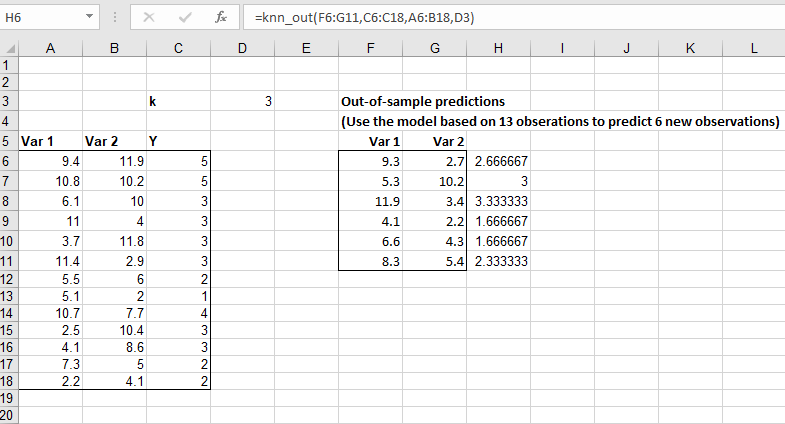
\includegraphics[width=4in]{figures/knnout4}}

\medskip
\end{enumerate}

\newpage

\subsection{K-Nearest Neighbor Functions (User-based)}

\textit{Tip:} The functions in this section do user-based prediction, which means that they predict a score (or rating) based on the scores of other users. These function do not use any other content-attribute (as movie characteristics). You should use these functions when you want to predict ratings (for example, movie ratings) based only on the ratings of other users.


\subsubsection{knn\_in\_movie}

\textit{The example illustrated below is available on the}  \href{https://www8.gsb.columbia.edu/bizanalytics/excel-add-in/multiplatform#h-4}{ \textit{add-in webpage}}
 \textit{by downloading the Classification, KNN, Misc file and going to the knn\_in\_movie sheet.}
 
\textbf{knn\_in\_movie} uses the \texttt{k}-nearest neighbor algorithm to make predictions within a specified sample of users' ratings.

To use the function:
\begin{enumerate}
\item Write the parameter \texttt{k} in an empty cell, \texttt{k}=3 in the example below; select the first cell in which you want the output to be displayed; call the function by typing \texttt{=knn\_in\_movie(} in the formula bar and then pressing the $\boldsymbol{f_x}$ symbol next to the formula bar.

\medskip

\centerline{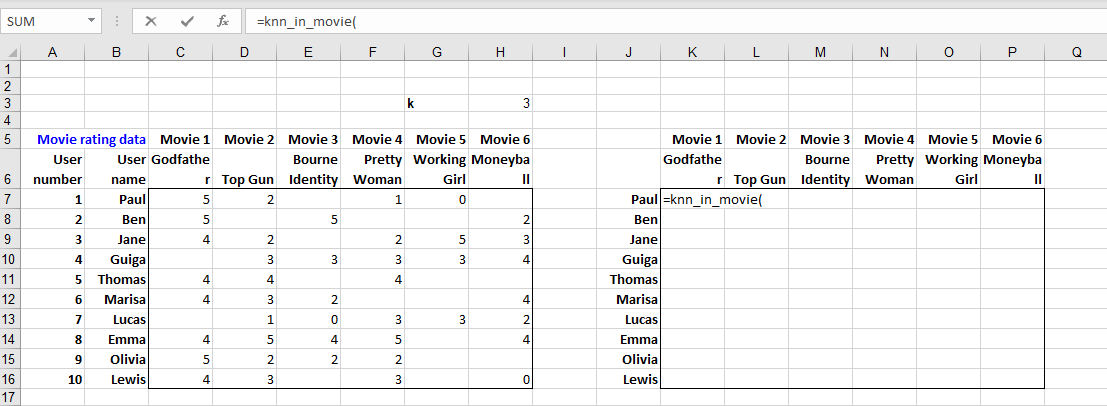
\includegraphics[width=5.5in]{figures/knninmovie1}}

\medskip

\item Follow the instructions to populate the input fields, as demonstrated in the figure below, then click \texttt{OK}.

\medskip

\centerline{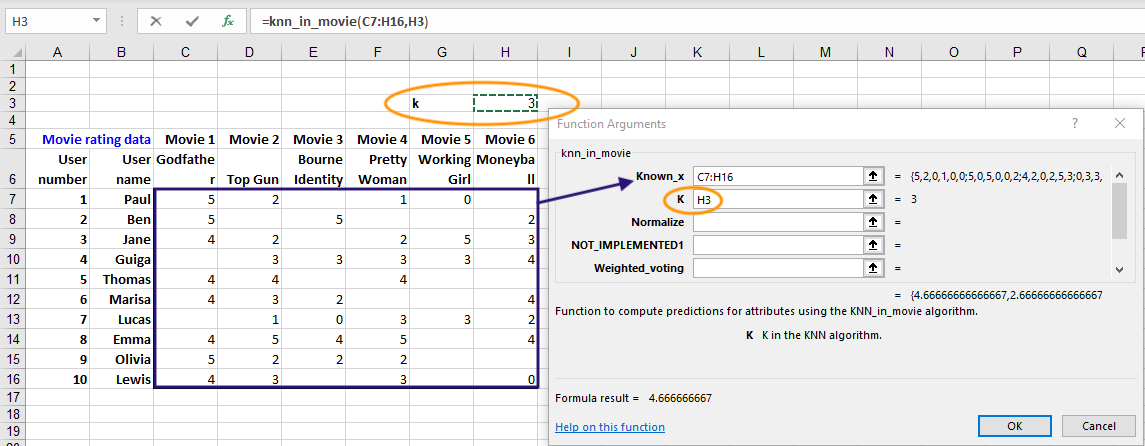
\includegraphics[width=5.5in]{figures/knninmovie2}}

\medskip

\item Remember that this is an array function. Select the area in which you want the output to be displayed: this should have the same number of rows and columns as the area that contains the users' ratings. In the figure below, we selected cells \texttt{K7:P16}.

\medskip

\centerline{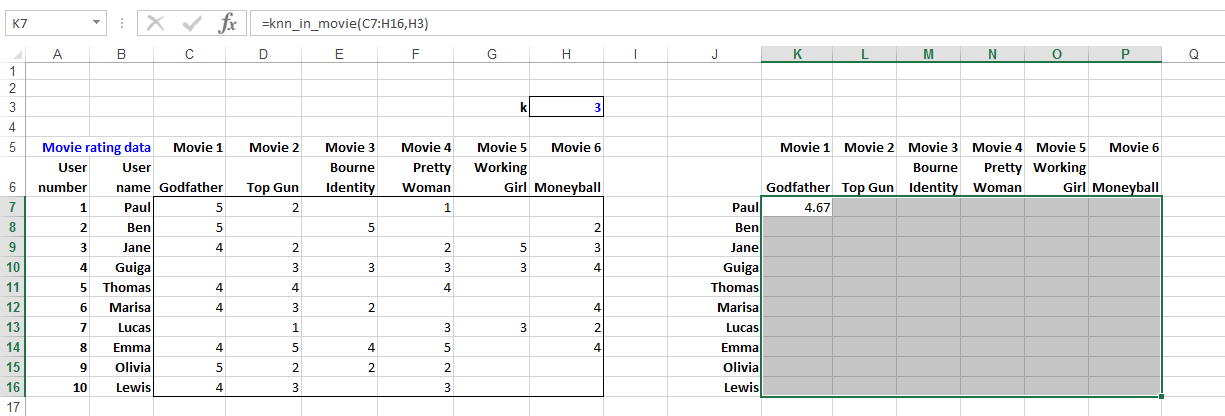
\includegraphics[width=5.8in]{figures/knninmovie3}}

\medskip

\item Position the cursor in the formula bar, and press \texttt{Ctrl+Shift+Enter} to display the predictions. You can also add a title to the output-column and format the output-cells to display only the first two decimals. \textit{Remark: for recent versions of Excel, this step is not necessary.}

\medskip

\centerline{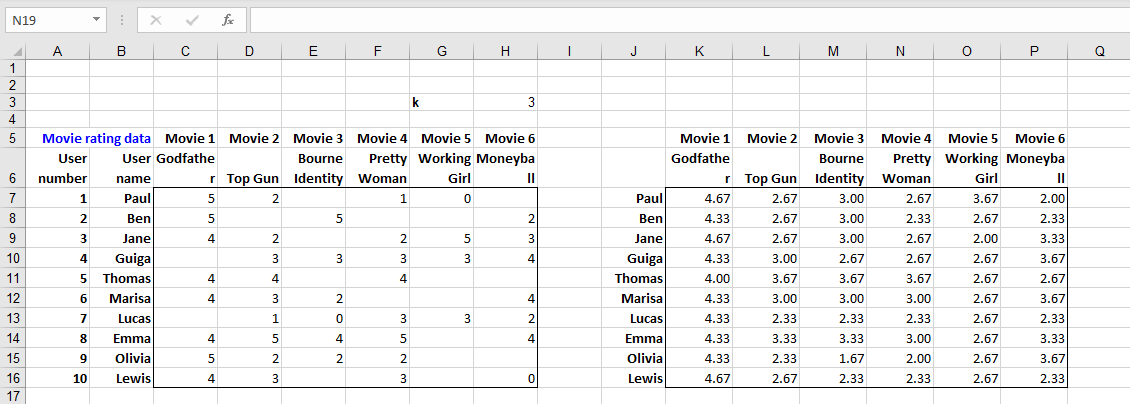
\includegraphics[width=5.8in]{figures/knninmovie4}}

\medskip
\end{enumerate}

\subsubsection{knn\_in\_movie\_rmse}

\textit{The example illustrated below is available on the}  \href{https://www8.gsb.columbia.edu/bizanalytics/excel-add-in/multiplatform#h-4}{ \textit{add-in webpage}}
 \textit{by downloading the Classification, KNN, Misc file and going to the knn\_in\_movie sheet.}

\textbf{knn\_in\_movie\_rmse} is a function that computes the Root Mean Squared Error (RMSE) for \text{k}-nearest neighbor predictions (as the ones you can obtain with \textbf{knn\_in\_movie}).


The inputs of the function are the users' ratings for a set of movies and the parameter \texttt{k} for which we want to compute the RMSE of predictions.

\textit{Note:} this is not an array function and can be evaluated in a single stand-alone cell, in which case it outputs the RMSE for a specified \text{k}. However, it is particularly useful when you want to compare RMSEs for different \text{k}. We will illustrate how to do this in the example below.

To use the function:
\begin{enumerate}
\item Write a list of parameters \texttt{k} for which you want to compute the RMSE, $\texttt{k}=1,2,...,9$ in the example below; select the cell next to the first value for \texttt{k}; call the function by typing \texttt{=knn\_in\_rmse(} in the formula bar and then pressing the $\boldsymbol{f_x}$ symbol next to the formula bar.

\medskip

\centerline{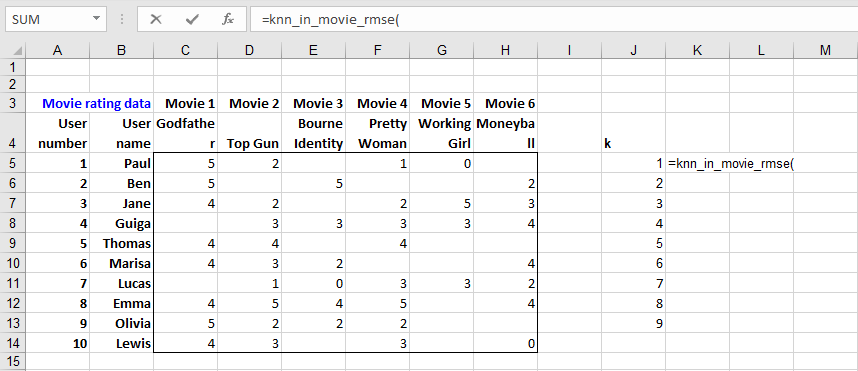
\includegraphics[width=4.5in]{figures/knninmoviermse1}}

\medskip

\item Input the references to the cells that contain the users' ratings, as in the figure below, then \textit{lock} the cell references with $\$$ signs. Input the reference of the cell that contains the first value for \texttt{k}, and make sure that this is \textit{not locked}. Then click \texttt{OK}.

\medskip

\centerline{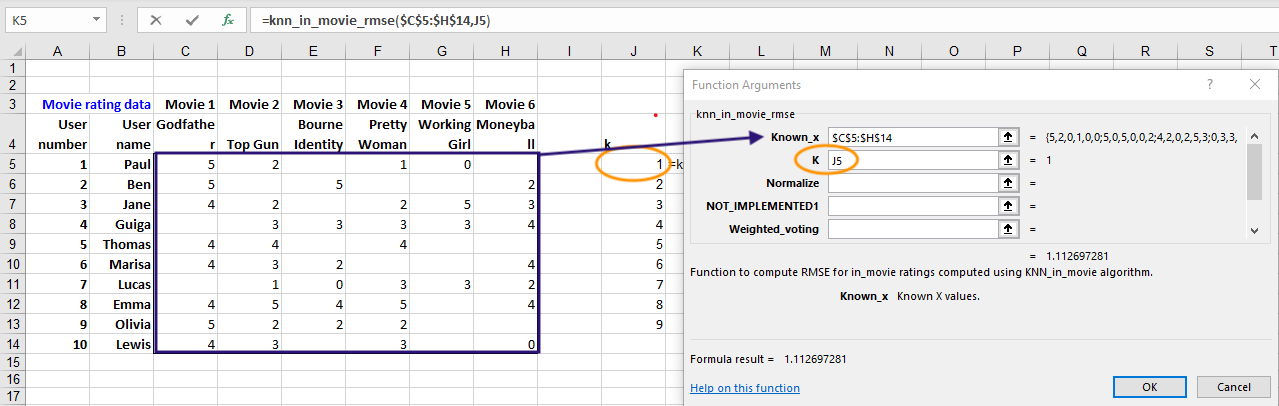
\includegraphics[width=5in]{figures/knninmoviermse2}}

\medskip

\item The function will display the output in the selected cell (\texttt{K5}). Copy the content of the cell down until cell \texttt{K13}, the formula will automatically update the calculation for every \texttt{k}. You can also format the output to display only three decimals.
\medskip

\centerline{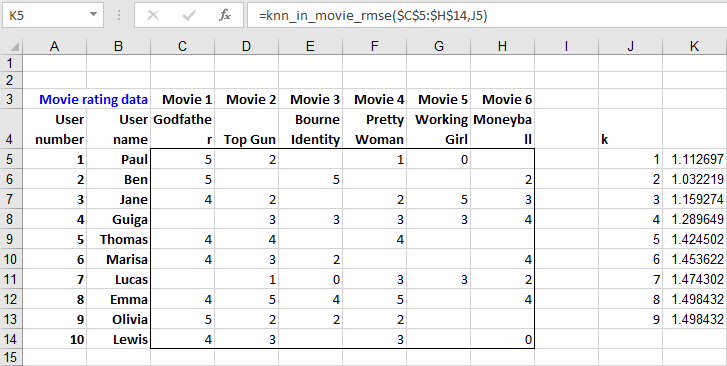
\includegraphics[width=4in]{figures/knninmoviermse3}}

\medskip
\end{enumerate}

% \subsubsection{knn\_out\_movie}

% \textit{The example illustrated below is in the cbs\_ba\_catalog excel file under the knn\_in\_movie sheet.}

% \textbf{knn\_out\_movie} uses the \texttt{k}-nearest neighbor algorithm to make predictions on users ratings for a new sample of movies based on users' ratings from an old sample of movies.

% To use the function:
% \begin{enumerate}
% \item Write the parameter \texttt{k} in an empty cell, \texttt{k}=3 in the example below. Select the first cell in which you want the output to be displayed; call the function by typing \texttt{=knn\_out\_movie(} in the formula bar and then pressing the $\boldsymbol{f_x}$ symbol next to the formula bar.

% \medskip

% \centerline{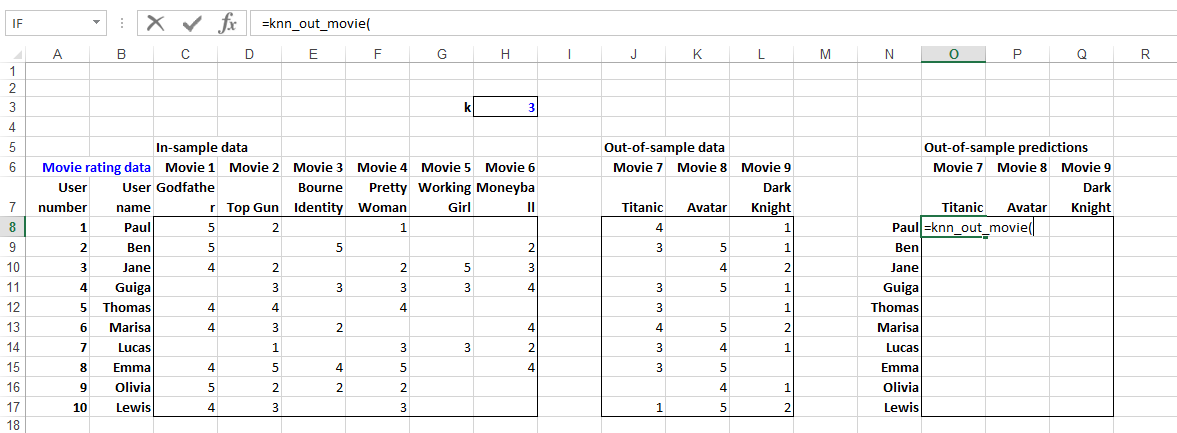
\includegraphics[width=5in]{figures/knnoutmovie1}}

% \medskip

% \item The function takes as inputs the new observations $X$, the old observations, and the parameter \texttt{k}. Follow the instructions to populate the input fields, as demonstrated in the figure below, then click \texttt{OK}.

% \medskip

% \centerline{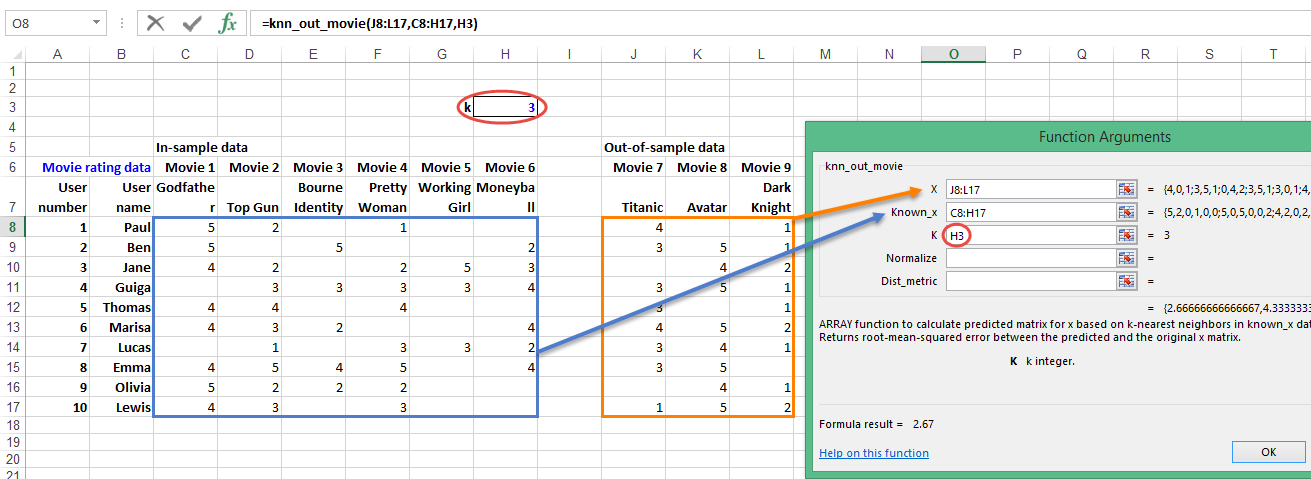
\includegraphics[width=5.8in]{figures/knnoutmovie2}}

% \medskip

% \item Remember that this is an array function. Select the area in which you want the output to be displayed: this should have the same dimensions as the new sample. In the example below we selected cells \texttt{O8:Q17}.

% \medskip

% \centerline{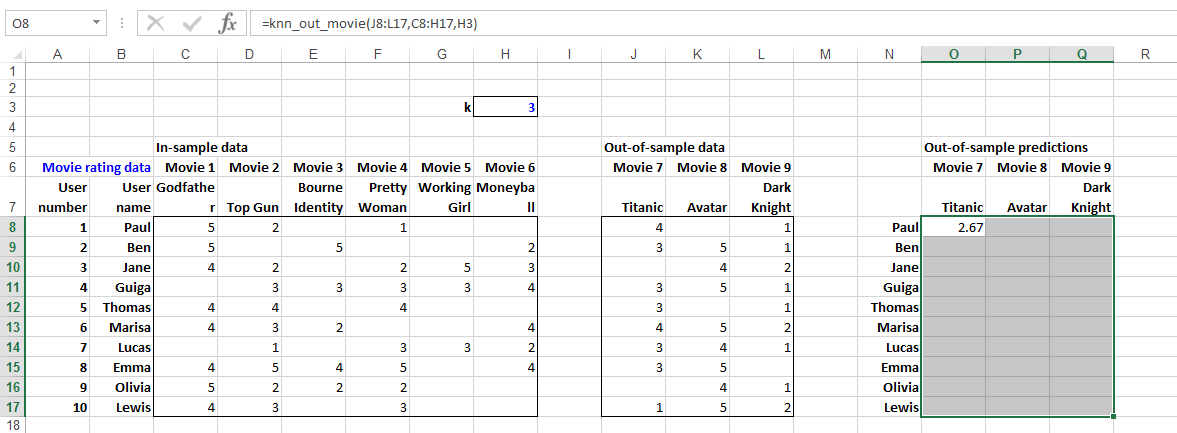
\includegraphics[width=5in]{figures/knnoutmovie3}}

% \medskip

% \item Position the cursor in the formula bar, and press \texttt{Ctrl+Shift+Enter} to display the predictions. You can also format the output to display only two decimals.

% \medskip

% \centerline{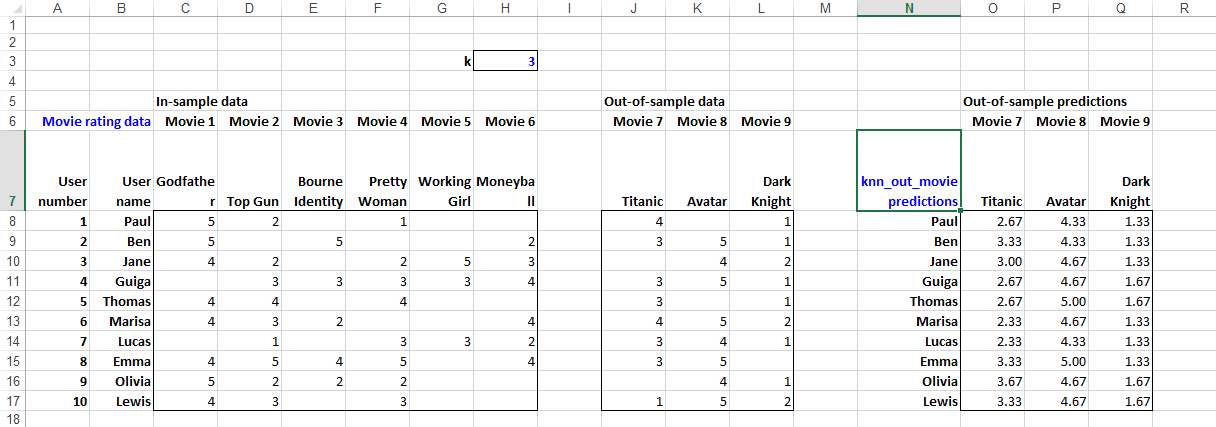
\includegraphics[width=5in]{figures/knnoutmovie4}}

% \medskip
% \end{enumerate}

% \newpage

\subsection{Other KNN Functions}

\textit{The example illustrated below is available on the}  \href{https://www8.gsb.columbia.edu/bizanalytics/excel-add-in/multiplatform#h-4}{ \textit{add-in webpage}}
 \textit{by downloading the Classification, KNN, Misc file and going to the knn\_full sheet.}

\subsubsection{knn\_dist}

\textbf{knn\_dist} is an array function that uses users' ratings to compute the distance of each user from a given user that you specify.

To use the function:
\begin{enumerate}
\item[0.] Decide the baseline user from which you want to compute the distances (we use \textbf{Jane} in the example below).
\item Select the first cell in which you want the output to be displayed; call the function by typing \texttt{=knn\_dist(} in the formula bar and then pressing the $\boldsymbol{f_x}$ symbol next to the formula bar.

\medskip

\centerline{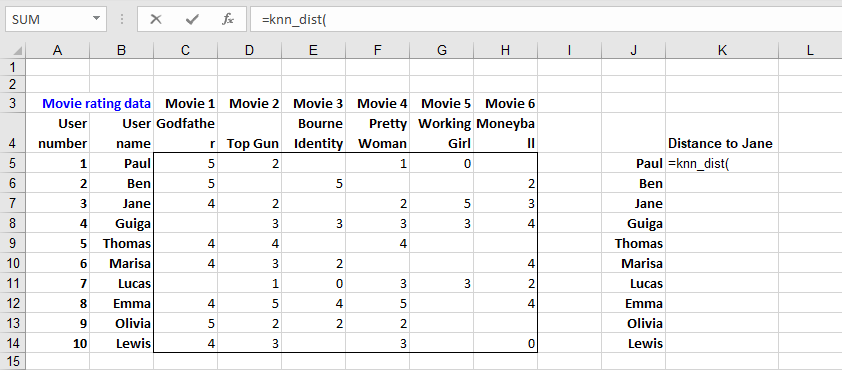
\includegraphics[width=4.5in]{figures/knndist1}}

\medskip

\item Follow the instructions to populate the input fields, as demonstrated in the figure below, then click \texttt{OK}.

\medskip

\centerline{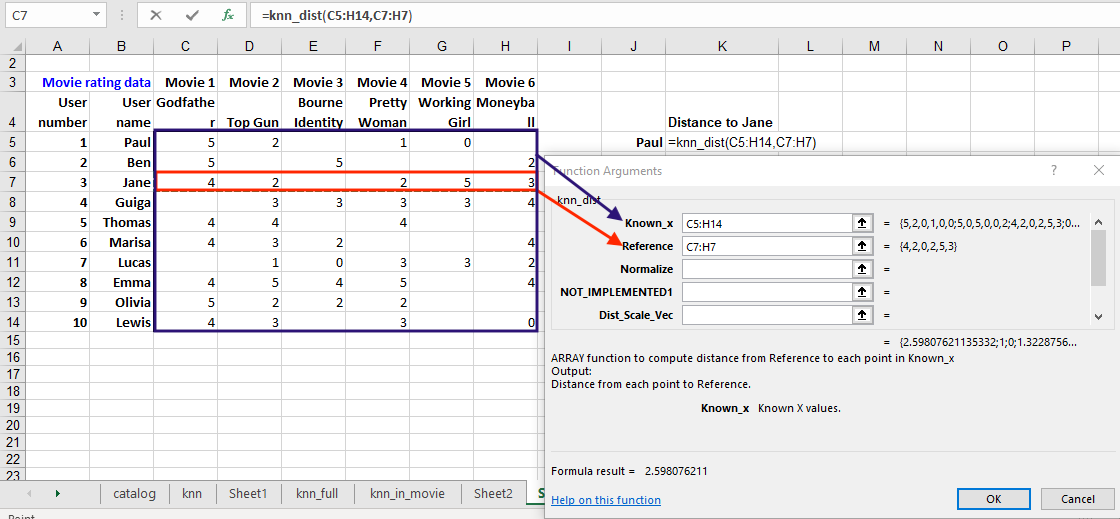
\includegraphics[width=5.5in]{figures/knndist2}}

\medskip

\item Remember that this is an array function. Select the column in which you want the output to be displayed: this should be a column of the same length as the number of users. In the figure below, we selected cells \texttt{K5:K14}.

\medskip

\centerline{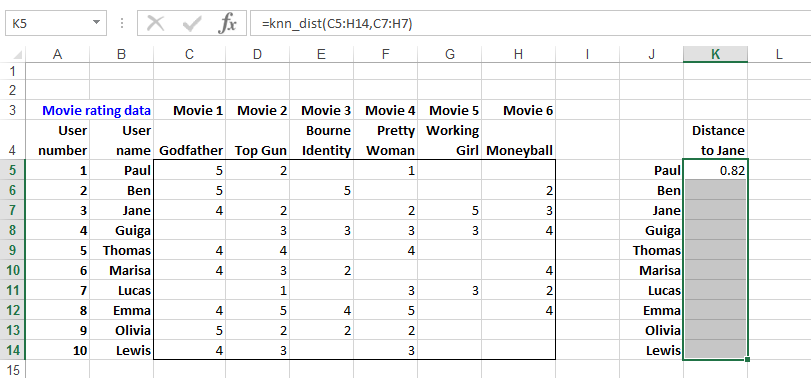
\includegraphics[width=4.5in]{figures/knndist3}}

\medskip

\item Position the cursor in the formula bar, and press \texttt{Ctrl+Shift+Enter} to display the predictions. You can also add a title to the output-column and format the output-cells to display only the first two decimals. \textit{Remark: for recent versions of Excel, this step is not necessary.}

\medskip

\centerline{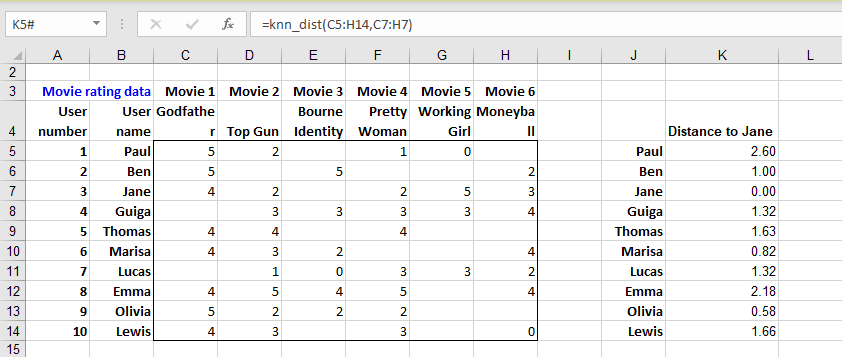
\includegraphics[width=4.5in]{figures/knndist4}}

\medskip
\end{enumerate}


\subsubsection{knn\_nearest}

\textbf{knn\_nearest} is an array function that uses users' ratings to rank users in order of
proximity (smallest distance) to a given user that you specify. The numbers returned are indices
of the rows in the input table in order of distance. (Note, in particular, that they are not
``ranks''.)

To use the function:
\begin{enumerate}
\item[0.] Decide the baseline user from which you want to compute the distance rankings (we use \textbf{Jane} in the example below).
\item Select the first cell in which you want the output to be displayed; call the function by typing \texttt{=knn\_nearest(} in the formula bar and then pressing the $\boldsymbol{f_x}$ symbol next to the formula bar.

\medskip

\centerline{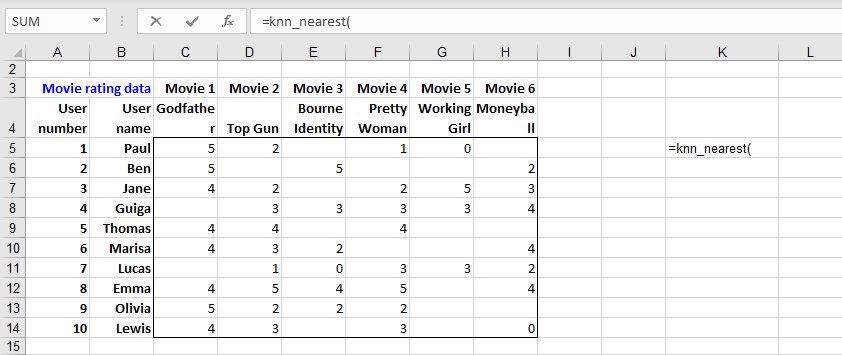
\includegraphics[width=4.5in]{figures/knnnearest1}}

\medskip

\item Follow the instructions to populate the input fields, as demonstrated in the figure below, then click \texttt{OK}.

\medskip

\centerline{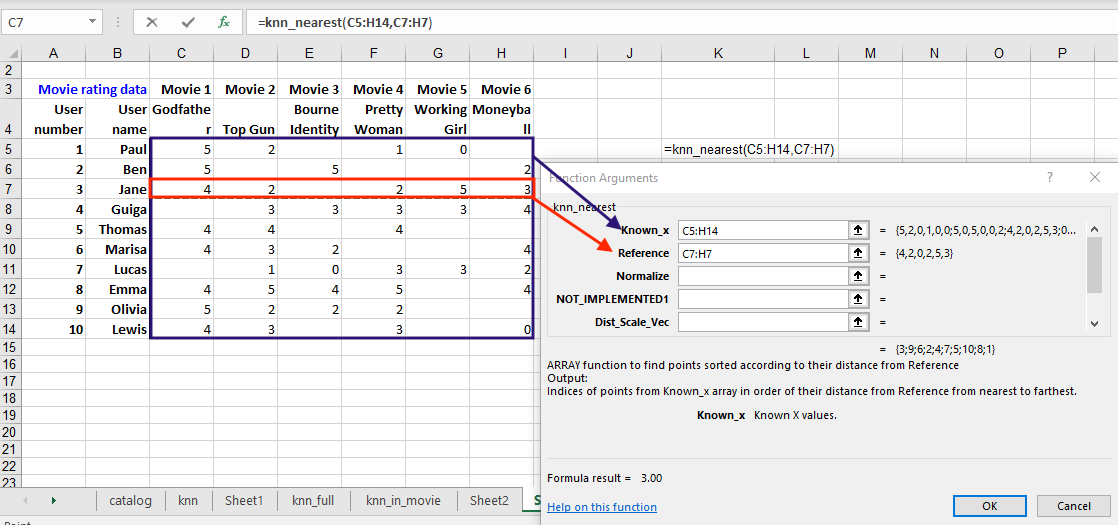
\includegraphics[width=5.5in]{figures/knnnearest2}}

\medskip

\item Remember that this is an array function. Select the column in which you want the output to be displayed: this should be a column of the same length as the number of users. In the figure below, we selected cells \texttt{K5:K14}.

\medskip

\centerline{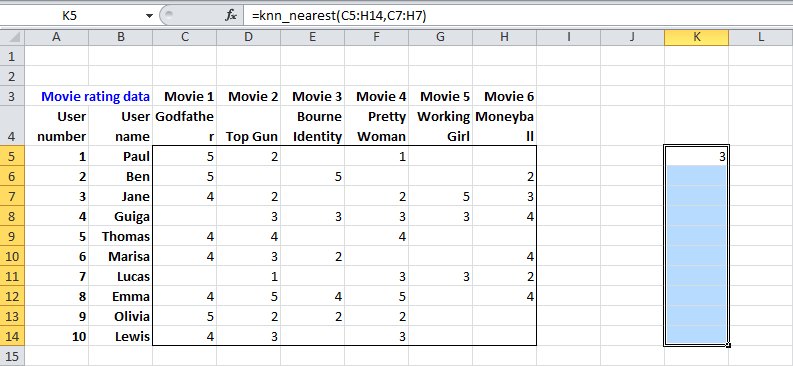
\includegraphics[width=4.5in]{figures/knnnearest3}}

\medskip

\item Position the cursor in the formula bar, and press \texttt{Ctrl+Shift+Enter} to display the predictions. You can also add a title to the output-column and format the output-cells to display the ranking without any decimals. \textit{Remark: for recent versions of Excel, this step is not necessary.}

\medskip

\centerline{\includegraphics[width=4.5in]{figures/knnnearest4}}

\end{enumerate}
To understand the output, consider the first number returned, 3. This means that the closest
person to Jane is the 3rd row (i.e., Jane herself). The second number is 9. This means the second
closest person is the 9th row (i.e., Olivia).

\medskip

\subsection{BA\_RMSE}

\textit{The example illustrated below is available on the}  \href{https://www8.gsb.columbia.edu/bizanalytics/excel-add-in/multiplatform#h-4}{ \textit{add-in webpage}}
 \textit{by downloading the Classification, KNN, Misc file and going to the ROC\_no\_cost sheet.}
 
 Suppose that you have access to $10$ experiments for which you observed \textbf{actual outcome} and the \textbf{predicted outcome} generated by some predictive model. 
 
 \centerline{\includegraphics[width=1.5in]{figures/rmse1}}

 
We illustrate in this section a function that computes the Root Mean Square Error.

To use the function:
\begin{enumerate}
\item Select the cell in which you want the output to be displayed; call the function by typing \texttt{=BA\_RMSE(} in the formula bar and then pressing the $\boldsymbol{f_x}$ symbol next to the formula bar.
\medskip

\centerline{\includegraphics[width=3.5in]{figures/rmse2.png}}

\medskip

\item Follow the instructions to populate the inputs of the function.

\medskip
\centerline{\includegraphics[width=3.5in]{figures/rmse3.png}}


\medskip

\item Click \texttt{OK} to display the result, in the example we have \textbf{RMSE=0.42}.


\end{enumerate}

\subsection{Classification Functions}

In this section we will illustrate a set of functions that you can use to solve classification problems. All the examples will be built upon the following dataset. Suppose that you have access to 17 experiments (e.g. clinical tests, spam/non-spam email classification, etc.) for which you observe the \textbf{actual outcome} of the experiment (1 if successful and 0 if not successful) and the \textbf{probability of success} generated by some predictive model.

\medskip

\centerline{\includegraphics[width=1.2in]{figures/conf1.png}}

\medskip

\subsubsection{confusionMatrix}

\textit{The example illustrated below is available on the}  \href{https://www8.gsb.columbia.edu/bizanalytics/excel-add-in/multiplatform#h-4}{ \textit{add-in webpage}}
 \textit{by downloading the Classification, KNN, Misc file and going to the ROC\_no\_cost sheet.}

Before illustrating the function, we build a classifier on the above dataset with a classification threshold of $0.6$: we predict as successful (1) the experiments that have a probability of success of at least $0.6$ and not successful (0) the others.

\medskip

\centerline{\includegraphics[width=2in]{figures/conf2.png}}

\medskip
We will use \textbf{confusionMatrix} to compute the Confusion Matrix associated to the above classifier.

To use the function:
\begin{enumerate}

\item Select the first cell in which you want the output to be displayed; call the function by typing \texttt{=confusionMatrix(} in the formula bar and then pressing the $\boldsymbol{f_x}$ symbol next to the formula bar.

\item Follow the instructions to populate the input fields, as demonstrated in the figure below, then click \texttt{OK}. (The actual and predicted values must both be binary.)

\medskip

\centerline{\includegraphics[width=5.5in]{figures/conf3.png}}

\medskip

\item Remember that this is an array function. Select the set of cells in which you want the output to be displayed. In the figure below, we selected cells \texttt{E3:H7}. \textit{Remark: for recent versions of Excel, this step is not necessary.}

\medskip

\centerline{\includegraphics[width=4.5in]{figures/conf4.png}}

\medskip

\item Position the cursor in the formula bar, and press \texttt{Ctrl+Shift+Enter} to display the output. You can also format the output-cells to display the labels of the matrix in boldface.

\medskip

\centerline{\includegraphics[width=3in]{figures/conf5.png}}

\end{enumerate}

\subsubsection{ROC}

\textit{The example illustrated below is available on the}  \href{https://www8.gsb.columbia.edu/bizanalytics/excel-add-in/multiplatform#h-4}{ \textit{add-in webpage}}
 \textit{by downloading the Classification, KNN, Misc file and going to the ROC\_no\_cost sheet.}

An important measure for evaluating the performance of a given classification model is the error rate. For example, consider the confusion matrix calculated in the previous section: the classifier built using a threshold of $0.6$ has a \textit{false positive rate} of $1/8=12.5\%$ and a \textit{true positive rate} of $3/9=33.3\%$. The ROC curve is simply a plot of the true positive versus the false positive rate for different thresholds. Note that, in principle, one can use any score for classification purposes. In the example, the score used was the predicted probability, but any other score can be used as well. By varying the classification threshold, different (FPR, TPR) pairs result, and the ROC curve captures all possible achievable pairs using that particular score/classifier. The ROC curve is a useful tool when you are trying to decide which classification threshold you should select.

To use the function:
\begin{enumerate}

\item[0.] Insert in a column the list of threshold values you want to test.

\medskip

\centerline{\includegraphics[width=2in]{figures/roc1.png}}

\medskip

\item Select the cell immediately to the right of the first threshold value, and call the function by typing \texttt{=ROC(} in the formula bar and then pressing the $\boldsymbol{f_x}$ symbol next to the formula bar.

\item Follow the instructions to populate the input fields, as demonstrated in the figure below, then click \texttt{OK}. (For the ROC curve with ``Cost'' see section \ref{ROCcost} below.)

\medskip

\centerline{\includegraphics[width=5.5in]{figures/roc2.png}}

\medskip

\item Remember that this is an array function. Select the set of cells in which you want the output to be displayed.

\medskip

\centerline{\includegraphics[width=2in]{figures/roc3.png}}

\medskip

\item Position the cursor in the formula bar, and press \texttt{Ctrl+Shift+Enter} to display the output. You can also format the output-cells to display only three decimals. \textit{Remark: for recent versions of Excel, this step is not necessary.}

\medskip

\centerline{\includegraphics[width=2in]{figures/roc4.png}}

\medskip

\item You can easily plot the false positive and true positive rates to display the ROC curve. To generate the graph below: select the set of cells that display the output of the \textbf{ROC} function; then select \texttt{INSERT - Charts - Scatter - Scatter with straight lines}.

\medskip

\centerline{\includegraphics[width=3.5in]{figures/roc5.png}}

\medskip

\end{enumerate}


\subsubsection{AUC}

\textit{The example illustrated below is available on the}  \href{https://www8.gsb.columbia.edu/bizanalytics/excel-add-in/multiplatform#h-4}{ \textit{add-in webpage}}
 \textit{by downloading the Classification, KNN, Misc file and going to the ROC\_no\_cost sheet.}
 
This function computes the area under the ROC curve.

To use the function:
\begin{enumerate}
\item Select the cell in which you want the output to be displayed; call the function by typing \texttt{=AUC(} in the formula bar and then pressing the $\boldsymbol{f_x}$ symbol next to the formula bar.

\item Follow the instructions to populate the inputs of the function.

\medskip

\centerline{\includegraphics[width=3.5in]{figures/auc.png}}

\medskip

\item Click \texttt{OK} to display the result, in the example we have \textbf{AUC=0.71}.

\end{enumerate}

\subsubsection{ROC (with cost information)}\label{ROCcost}

\textit{The example illustrated below is available on the}  \href{https://www8.gsb.columbia.edu/bizanalytics/excel-add-in/multiplatform#h-4}{ \textit{add-in webpage}}
 \textit{by downloading the Classification, KNN, Misc file and going to the ROC\_with\_cost sheet.}
 

This is a variation on the basic \textbf{ROC} function, when you have a cost associated to each type of classification error. The costs must be expressed in terms of a cost matrix.

\medskip

\centerline{\includegraphics[width=4.5in]{figures/roccost1.png}}

\medskip

To use the function follow the same steps as the basic \textbf{ROC} function, with the following variations:
\begin{itemize}
\item At \textit{Step 2.} insert also the cost matrix information: type \texttt{J6:K7} in the \texttt{Cost} input field.
\item At \textit{Step 3.} select three columns, as the function now outputs also the total cost. \textit{Remark: for recent versions of Excel, this step is not necessary.}
\medskip

\centerline{\includegraphics[width=2.5in]{figures/roccost2.png}}

\medskip
\end{itemize}
\medskip

\subsection{Monte Carlo Simulation}

In this section we will illustrate how to run a Monte Carlo Simulation in a spreadsheet.

%Before setting up the simulation, make sure you have all your add-in related files under the same folder, with names unchanged and no other files in that folder. In particular, the file \texttt{cbs\_ba\_hist.xlam} should be in the same folder as your \texttt{cbs\_ba.xll} file (or your \texttt{cbs\_ba64.xll} file). Also, make sure the BA add-in is enabled in your excel session.

\textit{The example illustrated below is available on the}  \href{https://www8.gsb.columbia.edu/bizanalytics/excel-add-in/multiplatform#h-4}{ \textit{add-in webpage}}
 \textit{by downloading the Monte Carlo Simulation file and going to the MCSim sheet.}

\textbf{Example: simple revenue simulation.} Suppose that you have 100 customers coming into your shop on each day and that each customer purchases something with probability 40\%. The accrued revenue per purchase is normally distributed with a mean of \$20 and a standard deviation of \$5. Simulate the \textbf{number of purchases}, the \textbf{revenue per purchase}, and the \textbf{total revenues}. Run the simulation for 500 trials.

To set up the simulation:

\begin{itemize}
\item[S0.] Populate the spreadsheet with the given data.

\centerline{\includegraphics[width=4in]{figures/simul1.png}}

\item[S1.] Insert the formulas for the quantities you want to simulate.

\begin{itemize}
\item[(S1.i)] Number of purchases: this is a random sample from a Binomial distribution with 100 trials and probability equal to $0.4$. You can use the add-in function \texttt{BinomSim} to generate this number.

\centerline{\includegraphics[width=4.5in]{figures/simul2.png}}

\item[(S1.ii)] Revenue per purchase: this is a random sample from a Normal distribution with mean 20 and standard deviation 5. You can use the add-in function \texttt{NormalSim} to generate this number.

\centerline{\includegraphics[width=4.5in]{figures/simul3.png}}

\item[(S1.ii)] Total Revenues: this is simply the product of number of purchases times revenue per purchase. Select cell \texttt{B13} and insert the formula \texttt{=B7$^*$B11}.
\end{itemize}

\item [S2.] Create the formula row, which will be your input for the simulation. Simply copy and paste the formulas from (1.i), (1.ii) and (1.iii) to an empty row. We did this in the figure below, in particular we inserted \texttt{=B7} in cell \texttt{E5}, \texttt{=B11} in cell \texttt{F5}, and \texttt{=B13} in cell \texttt{G5}.

\centerline{\includegraphics[width=4.5in]{figures/simul4.png}}

\item[S3.] You can also add an (optional) row of labels which indicates the variable for which you would like an histogram to be automatically generated, along with the simulation results. In our example we insert a row of labels with 0s for the first two variables and 1 for \textbf{total revenues}. As a result an histogram for this last variable will be generated, along with the simulation results.


\medskip

\vspace*{.1cm}
\centerline{\includegraphics[width=3in]{figures/simul5.png}}
\end{itemize}

To run the simulation:

\begin{itemize}
\item[R0.] Go to the \texttt{CBS BA ADD-IN} tab and then select the \texttt{Monte Carlo Simulation} to pop up the \texttt{MonteCarlo Simulation Dialog}. (Alternatively, the  dialog can be popped up by clicking \texttt{Ctrl+Shift+M}.)

\medskip

\centerline{\includegraphics[width=4in]{figures/simul0.png}}

\item[R1.] Populate the inputs of the function in the \texttt{Dialog Box} and then click \texttt{OK}. Also, by selecting the \texttt{Print Histogram} check box you can automatically generate histograms of the selected variables. Note that the simulation can track any number of variables in a single row, not just the three used in this example.

\centerline{\includegraphics[width=4.5in]{figures/simul6.png}}
\end{itemize}

You can format the output of the simulation to display nicely as in the figure below.

\medskip

\centerline{\includegraphics[width=4.5in]{figures/simul7.png}}

In separate sheets the macro outputs the histograms. As an example, we present the histogram of \textbf{total revenues}.

\medskip

\centerline{\includegraphics[width=4.5in]{figures/simul8.png}}

You can use \texttt{CBS BA Add-In | Clear histogram sheets} to clear previously created histogram sheets.



%
%\subsection{Portfolio Optimization}
%
%\subsubsection{mean\_variance}
%
%\textit{The example illustrated below is in the cbs\_ba\_catalog excel file (accessible via Add-Ins > CBS\_ba Help > Catalog in Excel) under the mv sheet.}
%
%This function essentially solves an optimization problem:
%
%Given a \textit{set of assets}, \textit{expected returns} and \textit{standard deviation of returns} for each asset, and a \textit{correlation matrix} for asset returns, it computes optimal portfolio weights for each asset. The optimal weights \textit{maximize expected portfolio returns} subject to a constraint on the \textit{portfolio standard deviation} that the user specifies. The function outputs: (i) Portfolio expected returns; (ii) Portfolio standard deviation of returns; (iii) Optimal portfolio weights for each asset.
%
%\medskip
%
%\centerline{\includegraphics[width=5.5in]{figures/mv1.png}}
%
%\medskip
%
%To use the function:
%\begin{enumerate}
%
%\item[0.] Gather all input information in a single sheet, as in the figure above.
%
%\item Select the first cell in which you want the output to be displayed (\texttt{L3} in the example); call the function by typing \texttt{=mean\_variance(} in the formula bar and then pressing the $\boldsymbol{f_x}$ symbol next to the formula bar.
%
%\item Follow the instructions to populate the input fields, as demonstrated in the figure below, then click \texttt{OK}\footnote{Scroll down and check you filled all the parameters.}.
%
%\medskip
%
%\centerline{\includegraphics[width=5.5in]{figures/mv3.png}}
%
%\medskip
%
%\item Remember that this is an array function. Select the set of cells in which you want the output to be displayed. This function returns a column of values, with the output size being (two plus the number of assets).  In this case the output contains $2+6=8$ values since there are $6$ assets. The output contains the performance and composition of the optimal portfolio: its expected returns, its standard deviation, and the proportion of each asset.
%
%\medskip
%
%\centerline{\includegraphics[width=2in]{figures/mv2.png}}
%
%\medskip
%
%\item Position the cursor in the formula bar, and press \texttt{Ctrl+Shift+Enter} to display the output. You can also format the output-cells to display percentages and only two decimals.
%
%\medskip
%
%\centerline{\includegraphics[width=2in]{figures/mv4.png}}
%
%\medskip
%\end{enumerate}

\end{document}

%%% Local Variables:
%%% mode: latex
%%% TeX-master: t
%%% End:
